% !TeX spellcheck = sp
\documentclass[a4paper,11pt]{article}
%\documentclass[a4paper,twoside,11pt,titlepage]{book}
\usepackage[utf8]{inputenc}
\usepackage[spanish]{babel}
\usepackage{tikz}
\usepackage{tikz-cd}
\usetikzlibrary{babel}
%\usepackage[round]{natbib}
\usepackage[backend=bibtex,citestyle=alphabetic]{biblatex}
\addbibresource{bibliography/bibliography.bib}
\usepackage{float}
\usepackage{tikz-3dplot}
\usepackage[toc,page]{appendix}
\usetikzlibrary{patterns}
\usetikzlibrary{calc}
\usepackage{pgfplots}
\usetikzlibrary{external}
\usepackage{amsmath,amsthm,amssymb}
\usepackage{caption}
\usepackage{subcaption}

\usepackage{hyperref}
\usepackage{xcolor}

\hypersetup{
    colorlinks,
    citecolor=black,
    filecolor=black,
    linkcolor=black,
    urlcolor=black
}

\usepackage{minted}
\definecolor{monokaibg}{HTML}{272822}
\definecolor{friendlybg}{HTML}{f0f0f0}

% \usepackage[style=list, number=none]{glossary} %
%\usepackage{titlesec}
%\usepackage{pailatino}

\graphicspath{{img/}}
\decimalpoint
\usepackage{dcolumn}
\newcolumntype{.}{D{.}{\esperiod}{-1}}
\makeatletter
\addto\shorthandsspanish{\let\esperiod\es@period@code}
\makeatother


%\usepackage[chapter]{algorithm}
\RequirePackage{verbatim}
%\RequirePackage[Glenn]{fncychap}
\usepackage{fancyhdr}
\usepackage{graphicx}
\usepackage{afterpage}

\usepackage{longtable}
 
% ********************************************************************
% Re-usable information
% ********************************************************************
\newcommand{\myTitle}{P1-Navarro-Ramírez-Pilar.pdf\xspace}
\newcommand{\myDegree}{Grado en Ingeniería Informática y Matemáticas\xspace}
\newcommand{\myName}{Pilar Navarro Ramírez\xspace}
%\newcommand{\myProf}{M. Jesús García-Ligero Ramírez\xspace}
%\newcommand{\myOtherProf}{Carlos Ureña Almagro\xspace}
\newcommand{\myFaculty}{Escuela Técnica Superior de Ingenierías Informática y de
Telecomunicación\xspace}
\newcommand{\myFacultyShort}{E.T.S. de Ingenierías Informática y de
Telecomunicación\xspace}
\newcommand{\myUni}{\protect{Universidad de Granada}\xspace}
\newcommand{\myLocation}{Granada\xspace}
\newcommand{\myTime}{\today\xspace}
\newcommand{\myVersion}{Version 0.1\xspace}

\hypersetup{
pdfauthor = {\myName antoniogamiz10@gmail.com},
pdftitle = {\myTitle},
pdfsubject = {},
pdfkeywords = {raytracing, montecarlo, random, numbers},
pdfcreator = {pdflatex},
pdfproducer = {pdflatex}
}

%\hyphenation{}


%\usepackage{doxygen/doxygen}
\usepackage{url}
\usepackage{colortbl,longtable}
\usepackage[stable]{footmisc}
%\usepackage{index}

%\makeindex
%\usepackage[style=long, cols=2,border=plain,toc=true,number=none]{glossary}
% \makeglossary

% Definición de comandos que me son tiles:
%\renewcommand{\indexname}{Índice alfabético}
%\renewcommand{\glossaryname}{Glosario}

\pagestyle{fancy}
\fancyhf{}
\fancyhead[LO]{\leftmark}
\fancyhead[RE]{\rightmark}
\fancyhead[RO,LE]{\textbf{\thepage}}
%\renewcommand{\chaptermark}[1]{\markboth{\textbf{#1}}{}}
%\renewcommand{\sectionmark}[1]{\markright{\textbf{\thesection. #1}}}

\setlength{\headheight}{1.5\headheight}

\newcommand{\HRule}{\rule{\linewidth}{0.5mm}}
%Definimos los tipos teorema, ejemplo y definición podremos usar estos tipos
%simplemente poniendo \begin{teorema} \end{teorema} ...
%\newtheorem{theorem}{Teorema}[chapter]
%\newtheorem{example}{Ejemplo}[chapter]
%\newtheorem{definition}[chapter]{Definición}

\newcommand{\bigrule}{\titlerule[0.5mm]}


%Para conseguir que en las páginas en blanco no ponga cabecerass
\makeatletter
\def\clearpage{%
  \ifvmode
    \ifnum \@dbltopnum =\m@ne
      \ifdim \pagetotal <\topskip
        \hbox{}
      \fi
    \fi
  \fi
  \newpage
  \thispagestyle{empty}
  \write\m@ne{}
  \vbox{}
  \penalty -\@Mi
}
\makeatother

\usepackage{pdfpages}

\usepackage[a4paper, margin={1in}]{geometry}

\begin{document}

\begin{titlepage}
 
 
\newlength{\centeroffset}
\setlength{\centeroffset}{-0.5\oddsidemargin}
\addtolength{\centeroffset}{0.5\evensidemargin}
\thispagestyle{empty}

\noindent\hspace*{\centeroffset}\begin{minipage}{\textwidth}

\centering

\includegraphics[width=0.9\textwidth]{img/logo_ugr.jpg}\\[2cm]

\textsc{ \Huge Inteligencia de Negocio\\[1.5cm]}
\textbf{\textsc{ \huge Práctica 3:}}\\
 \huge  Competición en Kaggle\\[1cm]
% Upper part of the page
% 
% Title
%{\Huge\bfseries \\
%}
%\noindent\rule[-1ex]{\textwidth}{3pt}\\[3.5ex]
%{\large\bfseries }
\end{minipage}

\vspace{2cm}
\noindent\hspace*{\centeroffset}\begin{minipage}{\textwidth}
\centering

\textbf{Autor}\\[0.2cm] {Pilar Navarro Ramírez}\\[0.2cm]
pilarnavarro@correo.ugr.es \\[0.2cm]
Grupo de prácticas 1 \\[1cm]


\includegraphics[width=0.3\textwidth]{img/etsiit_logo.png}\\[0.1cm]
\textsc{Escuela Técnica Superior de Ingeniería Informática y de Telecomunicaciones}\\
\textsc{---}\\
Granada, 4 de enero de 2021
\end{minipage}
%\addtolength{\textwidth}{\centeroffset}
%\vspace{\stretch{2}}
\end{titlepage}



%\input{preface/preface}

%\tableofcontents
%\listoffigures
%\listoftables

\tableofcontents
\newpage


\section{Introducción}
En esta práctica se analizarán diferentes algoritmos de aprendizaje supervisado con el objetivo de llevar a cabo una clasificación de tumores de mama en malignos y benignos. Para ello se dispone de un conjunto de datos de pacientes, en el que aparecen los valores de distintas variables, casi todas de tipo categórico (código BI-RADS, edad, forma de la masa anormal, densidad, margen), que nos ayudarán a la clasificación, así como los tipos de tumores que posee cada paciente (las etiquetas de las clases). Usaremos el conjunto de datos para entrenar los distintos modelos y realizar predicciones para determinar la bondad de los mismos. 

Estudiaremos algunos de los clasificadores vistos en clase de teoría. En concreto, vamos a analizar los resultados obtenidos con máquinas lineales de soporte vectorial, el algoritmo de los k vecinos más cercanos, árboles de decisión, random forest y redes neuronales. 

Hemos elegido algunos de estos clasificadores siguiendo el mapa que nos proporciona \mintinline{python}{sklearn} para seleccionar el clasificador más apropiado en cada caso: 

\begin{figure}[H]
	\centering
	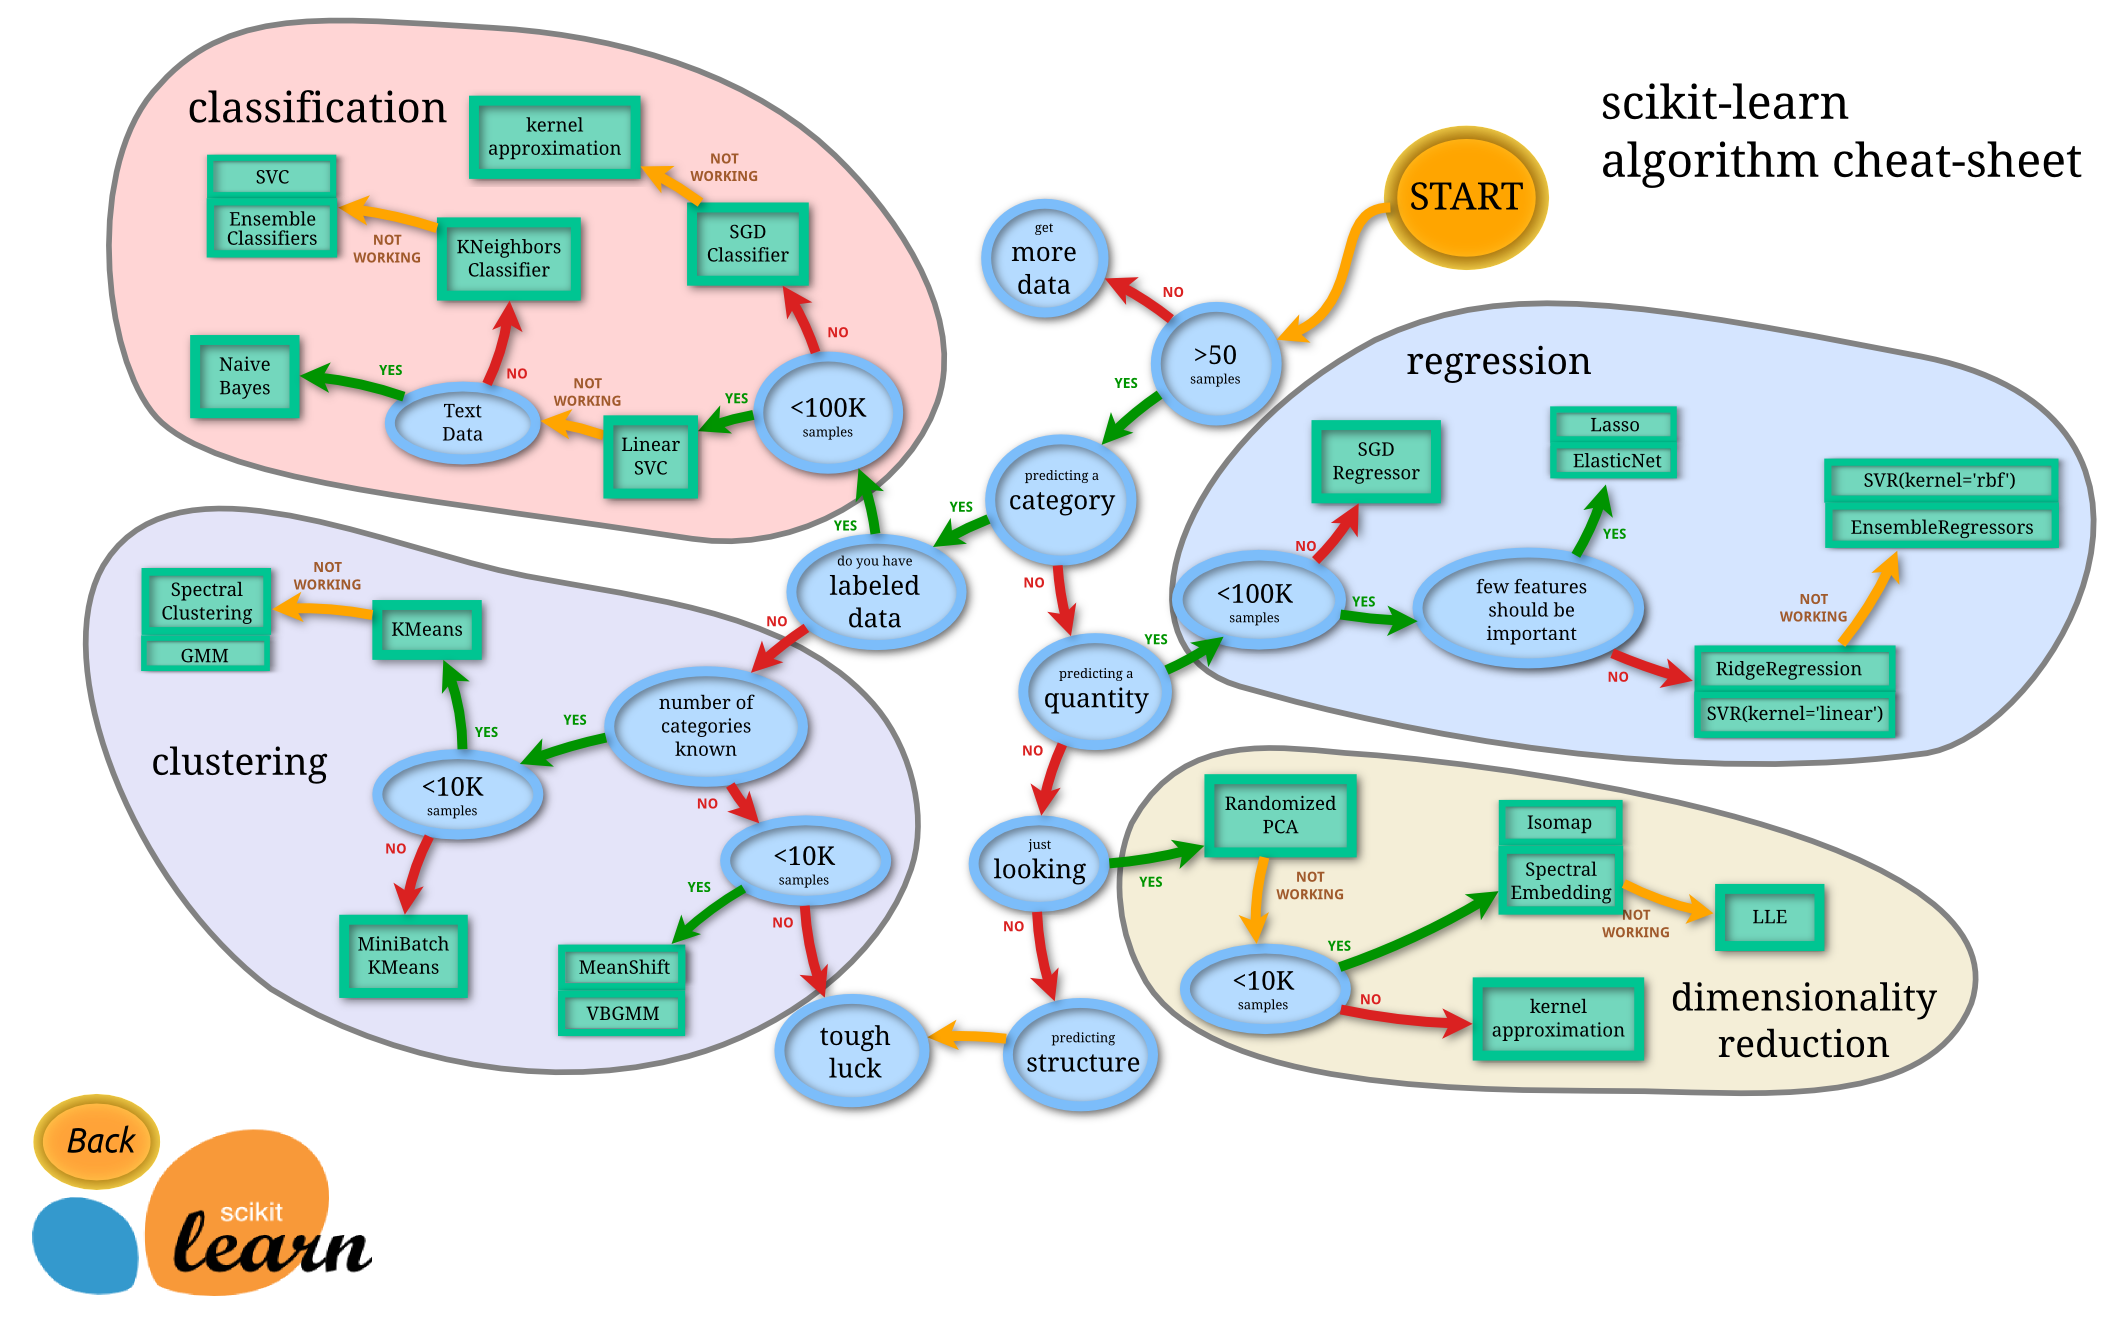
\includegraphics[width=1\linewidth]{img/map}
	\caption{}
	\label{fig:map}
\end{figure}

Como disponemos de más de 50 ejemplos (tenemos 961), vamos a predecir una categoría, nuestros datos están etiquetados y tenemos menos de 100.000 ejemplos llegamos a las máquinas de soporte vectorial lineales, que es uno de los clasificadores que hemos seleccionado. No sabemos a priori si va a funcionar, con lo que continuamos siguiendo el mapa, por si acaso. Nuestros ejemplos contienen datos de texto, pero en el preprocesamiento vamos a convertirlos en numéricos, con lo que el mapa nos lleva al algoritmo de los vecinos más cercanos. Finalmente, si volvemos a suponer que no va a funcionar, llegamos a los \textit{ensemble classifiers}, como es el Random Forest, que también vamos a estudiar. 

A parte de estos, consideramos los árboles de decisión por ser generalmente bastante eficientes y fáciles de utilizar. Además, tratan bien los datos con ruido, que puede ser que aparezca en nuestros ejemplos (lo cual tampoco sabemos al principio), así como con variables categóricas, que son con las que contamos. Pero sobre todo, los elegimos por ser uno de los modelos que se puede interpretar con mayor facilidad. Otro motivo por el que escogimos el algoritmo de Random Forest es que este suele mejorar los resultados proporcionados por los árboles de decisión, al considerar un conjunto de ellos y reducir el sobreaprendizaje en el que puede incurrir un sólo árbol. 

Finalmente, las redes neuronales son bien conocidas por proporcionar resultados bastante buenos en la mayoría de los problemas de clasificación y ser capaces de aprender conceptos complejos, que los árboles de decisión en cambio no podrían aprender. Por tanto, trabajaremos con ellas para ver si realmente son buenas también en nuestro estudio y comparar los resultados con los ofrecidos por los árboles de decisión. 


\newpage
\section{Procesado de datos}

En primer lugar, analizamos el conjunto de datos del que disponemos y realizamos distintos preprocesados con el fin de mejorar las predicciones llevadas a cabo por los distintos clasificadores que veremos más adelante. 


Empezamos obteniendo información de los datos en 'crudo' de que disponemos (\mintinline{python}{raw_data}), a través de la función \mintinline{python}{info()} que nos ofrece pandas:

\begin{figure}[H]
	\centering
	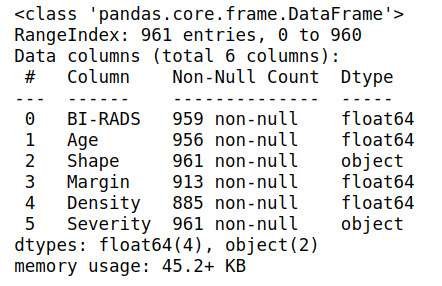
\includegraphics[width=0.7\linewidth]{img/image1}
	\caption{}
	\label{fig:image1}
\end{figure}

Podemos observar que todas las columnas (atributos) menos \textbf{Shape} y \textbf{Severity} tienen valores perdidos, pues hay menos de 961 (número total de instancias de las que disponemos) valores non-null en dichas columnas. Así pues, lo primero que tenemos que hacer es tratar con estos valores perdidos. Pero antes, puesto que tenemos atributos que no son numéricos, y algunos clasificadores con los que vamos a trabajar no tratan bien con strings, convertimos estos atributos a valores numéricos haciendo uso de la funcionalidad \mintinline{python}{preprocessing.LabelEncoder()} de \mintinline{python}{sklearn}. Obtenemos así el \mintinline{python}{Dataframe} que llamamos \mintinline{python}{numeric_data}

Usamos dos estrategias para lidiar con los datos perdidos.
\begin{enumerate}
	\item Primeramente, probamos la opción más sencilla que es eliminar las filas que tengan valores perdidos con la función \mintinline{python}{dropna()} de \mintinline{python}{pandas}. Como resultado obtenemos el \mintinline{python}{Dataframe} que llamamos \mintinline{python}{less_data}
	\item Como segunda opción, sustituimos los valores perdidos por el valor más fecuente de la columna correspondiente. Con este fin, utilizamos \mintinline{python}{SimpleImputer} de \mintinline{python}{sklearn.impute} y al resultado lo llamamos \mintinline{python}{replaced_data}.
\end{enumerate}

Otra posibilidad hubiera sido reemplazar los valores perdidos por la media de los valores de la columna afectada. Sin embargo, en nuestro caso esta opción no es muy apropiada pues tratamos con variables categóricas, a cuyos valores no es lógico calcularle la media. Es más lógico considerar la moda por ejemplo. 

Una vez que el problema de los valores perdidos ha sido solucionado parcialmente, aplicamos los distintos clasificadores considerados a los diversos \mintinline{python}{Dataframe} que hemos obtenido mediante este preprocesamiento. Para esto dejamos los hiperparámetros de los clasificadores con valores por defecto, y comparamos los resultados obtenidos para intentar determinar cual de las opciones nos da mejores predicciones. En las siguientes tablas podemos ver las salidas de las métricas de evaluación obtenidas con los distintos clasificadores para ambas opciones de preprocesamiento realizadas hasta ahora. 

\begin{table}[H]
	\caption{Accuracy}
	\centerline{
	\begin{tabular}{|c|r|r|r|r|r|}
		\hline
		\textbf{} & \multicolumn{1}{c|}{\textbf{Linear SVC}} & \multicolumn{1}{c|}{\textbf{kNN}} & \multicolumn{1}{c|}{\textbf{Árbol de decisión}} & \multicolumn{1}{c|}{\textbf{Random forest}} & \multicolumn{1}{c|}{\textbf{Red neuronal}} \\ \hline
		less\_data & 0.8252558301427 & 0.7981204316045 & 0.7779951270449 & 0.8087504350852 & 0.8016150365471 \\ \hline
		replaced\_data & 0.8323633832231 & 0.7993108249216 & 0.7839679777236 & 0.813470240167 & 0.8063487643578 \\ \hline
	\end{tabular}}
	\label{}
\end{table}

\begin{table}[H]
	\caption{AUC}
	\centerline{
	\begin{tabular}{|c|r|r|r|r|r|}
		\hline
		\textbf{} & \multicolumn{1}{c|}{\textbf{Linear SVC}} & \multicolumn{1}{c|}{\textbf{kNN}} & \multicolumn{1}{c|}{\textbf{Árbol de decisión}} & \multicolumn{1}{c|}{\textbf{Random forest}} & \multicolumn{1}{c|}{\textbf{Red neuronal}} \\ \hline
		less\_data & 0.825922795697 & 0.797888272147 & 0.7768099277338 & 0.8086506961702 & 0.80238703714 \\ \hline
		replaced\_data & 0.8321279762509 & 0.798296767384 & 0.779394817891 & 0.8150029742851 & 0.8082588929874 \\ \hline
	\end{tabular}}
	\label{}
\end{table}

\begin{table}[H]
	\caption{F1-score}
	\centerline{
	\begin{tabular}{|c|r|r|r|r|r|}
		\hline
		\textbf{} & \multicolumn{1}{c|}{\textbf{Linear SVC}} & \multicolumn{1}{c|}{\textbf{kNN}} & \multicolumn{1}{c|}{\textbf{Árbol de decisión}} & \multicolumn{1}{c|}{\textbf{Random forest}} & \multicolumn{1}{c|}{\textbf{Red neuronal}} \\ \hline
		less\_data & 0.8227365658017 & 0.7950620849451 & 0.7586725291309 & 0.8013035065117 & 0.8033646314783 \\ \hline
		replaced\_data & 0.8182631300244 & 0.7809578062902 & 0.7500298347871 & 0.7952746093769 & 0.7926877734449 \\ \hline
	\end{tabular}}
	\label{}
\end{table}

Podemos observar que con todos los clasificadores seleccionados, para la precisión y el AUC, los resultados son mejores con los datos en los que reemplazamos los valores perdidos por la moda de su columna. Esto es debido a que en este caso disponemos de más datos que, por el contrario, eliminamos en \mintinline{python}{less_data}. Sin embargo, para  el F1-score ocurre lo contrario. La diferencia está en que esta última métrica penaliza más los Falsos Negativos que las otras dos, lo cual nos indica que con \mintinline{python}{replaced_data} habrá generalmente más falsos negativos que con \mintinline{python}{less_data}. La diferencia es mínima, pero como en nuestro caso los falsos negativos son bastante importantes, debería haber los menos posibles (predecir que el tumor de un paciente es benigno cuando en realidad es maligno es un problema). Por lo tanto, deducimos que \mintinline{python}{less_data} será mejor en nuestro caso. 

Otro aspecto a tener en cuenta sería el balanceo de las clases. Los datos con los que trabajamos tienen un pequeño desbalance, pues hay más instancias de la clase benigna frente a la clase maligna (516 frente a 445)

\begin{figure}[H]
	\centering
	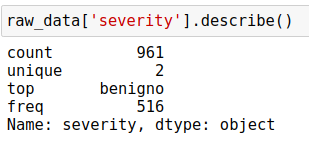
\includegraphics[width=0.7\linewidth]{img/image2}
	\caption{}
	\label{fig:image2}
\end{figure}

Sin embargo, teniendo en cuenta que disponemos de 961 instancias, este desbalance supone un $\frac{516-445}{961} * 100 = 7,4\%$. Es más, en los datos \mintinline{python}{less_data}, el desbalance es del $\frac{437-410}{847} * 100 = 3,2\%$ (ver Figura 3). Así pues, no merece la pena detenerse a tratar con este problema, pues la mejora (si acaso existente) sería mínima. 

\begin{figure}[H]
	\centering
	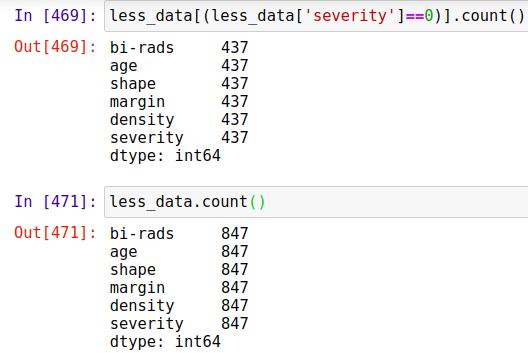
\includegraphics[width=0.9\linewidth]{img/image3}
	\caption{}
	\label{fig:image3}
\end{figure}

Analizamos ahora la correlación entre las variables usando la función \mintinline{python}{.corr()} de \mintinline{python}{pandas} y el coeficiente de correlación de Spearman. Obtenemos lo siguiente:

\begin{figure}[H]
	\centering
	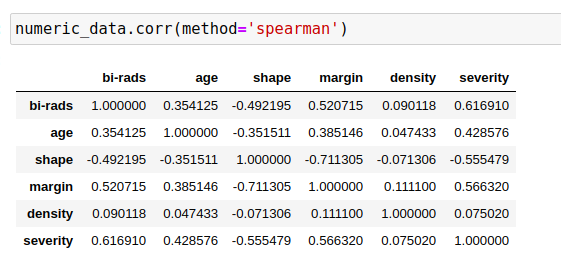
\includegraphics[width=1\linewidth]{img/image4}
	\caption{}
	\label{fig:image4}
\end{figure}

Podemos observar que los atributos \textbf{shape} y \textbf{margin} son los que están más correlacionados, pues el valor del coeficiente de correlación de Spearman es -0.71, lo cual está próximo a -1.
Así pues, probamos a eliminar uno de estos atributos. Como \textbf{margin} tiene más valores perdidos que \textbf{shape} (ver Figura 1) eliminamos su columna en vez de la de \textbf{shape} en \mintinline{python}{numeric_data}. De hecho, la columna de \textbf{margin} es de las que tienen más datos nulos, lo cual al eliminar este atributo también estamos resolviendo implícita y parcialmente el problema de los valores perdidos. A continuación, eliminamos las instancias que siguen teniendo datos perdidos con \mintinline{python}{dropna()} y el resultado lo almacenamos en \mintinline{python}{corr_data}. El resultado tras ejecutar \mintinline{python}{corr_data.info()} es el siguiente:

\begin{figure}[H]
	\centering
	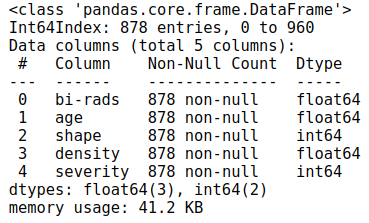
\includegraphics[width=0.7\linewidth]{img/image5}
	\caption{}
	\label{fig:image5}
\end{figure}

con lo que en este caso disponemos de más instancias (878) que en \mintinline{python}{less_data} (847). 

Analizamos entonces los resultados obtenidos para estos nuevos datos comparándolos con los que ya teníamos:

\begin{table}[htbp]
	\caption{Accuracy}
	\centerline{
	\begin{tabular}{|c|r|r|r|r|r|}
		\hline
		\textbf{} & \multicolumn{1}{c|}{\textbf{Linear SVC}} & \multicolumn{1}{c|}{\textbf{kNN}} & \multicolumn{1}{c|}{\textbf{Árbol de decisión}} & \multicolumn{1}{c|}{\textbf{Random forest}} & \multicolumn{1}{c|}{\textbf{Red neuronal}} \\ \hline
		less\_data & 0.8252558301427 & 0.7981204316045 & 0.7779951270449 & 0.8087504350852 & 0.8016150365471 \\ \hline
		replaced\_data & 0.8323633832231 & 0.7993108249216 & 0.7839679777236 & 0.813470240167 & 0.8063487643578 \\ \hline
		corr\_data & 0.8264462234597 & 0.7698085624782 & 0.7697737556561 & 0.7980577793247 & 0.793372781065 \\ \hline
	\end{tabular}}
	\label{}
\end{table}

\begin{table}[htbp]
	\caption{AUC}
	\centerline{
	\begin{tabular}{|c|r|r|r|r|r|}
		\hline
		\textbf{} & \multicolumn{1}{c|}{\textbf{Linear SVC}} & \multicolumn{1}{c|}{\textbf{kNN}} & \multicolumn{1}{c|}{\textbf{Árbol de decisión}} & \multicolumn{1}{c|}{\textbf{Random forest}} & \multicolumn{1}{c|}{\textbf{Red neuronal}} \\ \hline
		less\_data & 0.825922795697 & 0.797888272147 & 0.7768099277338 & 0.8086506961702 & 0.80238703714 \\ \hline
		replaced\_data & 0.8321279762509 & 0.798296767384 & 0.779394817891 & 0.8150029742851 & 0.8082588929874 \\ \hline
		corr\_data & 0.8256091918497 & 0.7687251803454 & 0.7688380621922 & 0.798553743736 & 0.794072350702 \\ \hline
	\end{tabular}}
	\label{}
\end{table}



\begin{table}[htbp]
	\caption{F1-score}
	\centerline{
	\begin{tabular}{|c|r|r|r|r|r|}
		\hline
		\textbf{} & \multicolumn{1}{c|}{\textbf{Linear SVC}} & \multicolumn{1}{c|}{\textbf{kNN}} & \multicolumn{1}{c|}{\textbf{Árbol de decisión}} & \multicolumn{1}{c|}{\textbf{Random forest}} & \multicolumn{1}{c|}{\textbf{Red neuronal}} \\ \hline
		less\_data & 0.8227365658017 & 0.7950620849451 & 0.7586725291309 & 0.8013035065117 & 0.8033646314783 \\ \hline
		replaced\_data & 0.8182631300244 & 0.7809578062902 & 0.7500298347871 & 0.7952746093769 & 0.7926877734449 \\ \hline
		corr\_data & 0.810525404177 & 0.7475747479002 & 0.7447295018394 & 0.7819330029314 & 0.7776191376369 \\ \hline
	\end{tabular}}
	\label{}
\end{table}


Es de notar que los resultados son peores para todas las medidas de evaluación y para todos los modelos con \mintinline{python}{corr_data}. Esto era de esperar, pues hemos eliminado uno de los atributos que aporta su propia información a los clasificadores. Aunque hemos visto que estaba correlaccionado con otra variable, el grado de correlacción no es suficiente como para poder prescindir de este atributo. La información que aporta ayuda al entrenamiento de los clasificadores así como a las predicciones, y esta información  propia  no puede ser extraída en su totalidad del otro atributo con el que está correlacionado. 

Concluimos por tanto, que de todos los preprocesamientos considerados para los datos de partida, el que ofrece mejores predicciones es en el caso en que eliminamos las instancias con valores perdidos y el resto de datos permanencen inalterados. Aunque ya hemos visto que las medidas de precisión y AUC son un poco peores para estos datos que para \mintinline{python}{replaced_data}, en nuestro estudio el F1-score es más importante. Teniendo en cuenta este criterio nos decidimos por \mintinline{python}{less_data}, de manera que a partir de ahora trabajaremos con estos datos para estudiar los distintos modelos.
 
\newpage
\section{Configuración de algoritmos}
\subsection{Vecinos más cercanos k-NN}

En el algoritmo de K-Nearest Neighbors el hiperparámtro más importante que debemos configurar es el número de vecinos, para evitar tanto el overfitting como el underfitting y llegar a un balance entre ambos. 

Sin embargo, antes de meternos a estudiar dicho parámetro consideramos otro par de aspectos. 

En primer lugar, como en nuestro caso las variables son nominales, la distancia que debemos usar es la de Hamming. En efecto, si comparamos los resultados obtenidos para esta distancia con los obtenidos para la distancia Euclídea (que es la que tiene el clasificador por defecto en \mintinline{python}{sklearn}) o la de Manhattan,  observamos que son mejores para la distancia de Hamming como era de esperar según las variables de las que disponemos:

\begin{table}[htbp]
	\caption{}
	\centerline{
	\begin{tabular}{|c|r|r|r|}
		\hline
		\multicolumn{1}{|l|}{} & \multicolumn{1}{c|}{\textbf{Euclidea}} & \multicolumn{1}{c|}{\textbf{Manhattan}} & \multicolumn{1}{c|}{\textbf{Hamming}} \\ \hline
		Accuracy & 0.798148277062304 & 0.795788374521406 & 0.802875043508528 \\ \hline
		AUC & 0.799843499482814 & 0.79579037233402 & 0.802405369259448 \\ \hline
		F1-score & 0.795453060494477 & 0.787051217927197 & 0.798243918126335 \\ \hline
	\end{tabular}}
	\label{}
\end{table}


Otro aspecto a tener en cuenta son los pesos asociados a los puntos en la 'vecindad'. El \mintinline{python}{KNeighborsClassifier}  de \mintinline{python}{sklearn} nos da dos opciones: 
\begin{itemize}
	\item Pesos uniformes para todos los puntos, es decir, todos los 'vecinos' tienen el mismo peso y su 'votación' tiene igual importancia. 
	\item Cada punto en el 'vecindario' tiene asociado un peso que es igual a la inversa de su distancia, de manera que puntos más cercanos a la instancia a clasificar tendrán mayor influencia en su 'voto' que los más lejanos.
\end{itemize}

Mostramos entonces los valores obtenidos en cada uno de los dos casos, haciendo uso tanto de la distancia de Hamming como de la Euclídea:

\begin{table}[htbp]
	\caption{Hamming Distance}
	\centerline{
	\begin{tabular}{|c|r|r|}
		\hline
		\multicolumn{1}{|l|}{} & \multicolumn{1}{c|}{\textbf{uniform}} & \multicolumn{1}{c|}{\textbf{distance}} \\ \hline
		Accuracy & 0.802875043508528 & 0.794604942568743 \\ \hline
		AUC & 0.802405369259448 & 0.793160693314314 \\ \hline
		F1-score & 0.798243918126335 & 0.772812544880101 \\ \hline
	\end{tabular}}
	\label{}
\end{table}

\begin{table}[H]
	\caption{Euclidean Distance}
	\centerline{
	\begin{tabular}{|c|r|r|}
		\hline
		\textbf{} & \multicolumn{1}{c|}{\textbf{uniform}} & \multicolumn{1}{c|}{\textbf{distance}} \\ \hline
		Accuracy & 0.798148277062304 & 0.785130525583014 \\ \hline
		AUC & 0.799843499482814 & 0.784532897126519 \\ \hline
		F1-score & 0.795453060494477 & 0.77428087698699 \\ \hline
	\end{tabular}}
	\label{}
\end{table}


Es claro que en todos los casos los resultados con pesos uniformes son mejores. Esto puede ser debido a que si asignamos pesos mayores a los vecinos más cercanos y menores a los más lejanos, se produce un sobreajuste a los datos de entrenamiento y las predicciones de nuevas instancias son, por tanto, peores. 

En cuanto al algoritmo para computar las distancias vamos a usar en todos los casos la opción 'auto', es decir, consideraremos \mintinline{python}{algorithm='auto'} que es la opción por defecto en \mintinline{python}{KNeighborsClassifier}, puesto que con esta opción se decide automáticamente cuál es el procedimiento óptimo en cada caso. 

Finalmente pasamos a estudiar lo prometido, el valor próximo al óptimo del número de vecinos. Para ello, escogemos los parámetros que nos han dado mejores resultados hasta ahora, es decir, distancia de Hamming y  pesos uniformes. Empezamos probando algunos valores y analizamos los resultados:

\begin{table}[htbp]
	\caption{}
	\centerline{
	\begin{tabular}{|c|r|r|r|r|r|}
		\hline
		K= & \multicolumn{1}{c|}{\textbf{1}} & \multicolumn{1}{c|}{\textbf{4}} & \multicolumn{1}{c|}{\textbf{5}} & \multicolumn{1}{c|}{\textbf{10}} & \multicolumn{1}{c|}{\textbf{20}} \\ \hline
		Accuracy & 0.7674625826662 & 0.77805081796 & 0.8028750435085 & 0.8205290636964 & 0.8169926905673 \\ \hline
		AUC & 0.7669300375132 & 0.774348635354 & 0.8024053692594 & 0.818006848172 & 0.8139154740686 \\ \hline
		F1-score & 0.7502044643505 & 0.72789437857 & 0.7982439181263 & 0.7964676565788 & 0.7930761427363 \\ \hline
	\end{tabular}}
	\label{}
\end{table}


Cuando el número de vecinos es demasiado pequeño se produce un sobreajuste a los datos de entrenamiento, de manera que instancias nuevas que no se encuentren en el conjunto de entrenamiento serán clasificadas incorrectamente la mayoría de las veces. Así pues, para un sólo vecino los resultados son los peores. Conforme aumentamos el número de vecinos los resultados van mejorando, hasta llegar a $k=10$ cuando las medidas de evaluación nos muestran los mejores datos. Para $k=20$ empiezan a empeorar los resultados, lo cual indica que el valor óptimo debería estar situado entre $k=5$ y $k=20$. Para valores mayores de $k$ los resultados no pueden mejorar, pues en ese caso nos encontramos con underfitting, y ni los datos de entrenamiento serían bien clasificadors. Por lo tanto hay que encontrar un equilibrio, que aquí hemos visto que se encuentra en torno a $k=10$. Probamos pues con más valores de $k$:

\begin{table}[htbp]
	\caption{}
\centerline{
	\begin{tabular}{|c|r|r|r|r|r|r|}
		\hline
		K= & \multicolumn{1}{c|}{\textbf{6}} & \multicolumn{1}{c|}{\textbf{7}} & \multicolumn{1}{c|}{\textbf{8}} & \multicolumn{1}{c|}{\textbf{10}} & \multicolumn{1}{c|}{\textbf{15}} & \multicolumn{1}{c|}{\textbf{17}} \\ \hline
		Accuracy & 0.81816219979 & 0.82293769578 & 0.82171945701 & 0.82052906369 & 0.81819700661 & 0.80989906021 \\ \hline
		AUC & 0.8174518844 & 0.82120374887 & 0.81969901731 & 0.8180068481 & 0.81549897193 & 0.80808710658 \\ \hline
		F1-score & 0.79462484659 & 0.8031505451 & 0.79966305526 & 0.79646765657 & 0.7999403271 & 0.78885278189 \\ \hline
	\end{tabular}}
	\label{}
\end{table}


Podemos afirmar entonces que con $k=7$ las predicciones son lo mejor posible. 

En resumen, hemos visto que para el algoritmo de k-NN y los datos de los que disponemos, la mejor configuración se obtiene considerando la distancia de Hamming, pesos uniformes y $k=7$, esto es, considerando las clases asociadas a los 7 vecinos más cercanos y seleccionando la clase mayoritaria entre ellos como predicción para una nueva instancia a clasificar. 

\subsection{Árboles de decisión}

Entramos ahora a estudiar los parámetros de este clasificador. El   \mintinline{python}{DecisionTreeClassifier} de \mintinline{python}{sklearn} dispone de numerosos parámetros que podemos configurar, aunque aquí nos centraremos sólo en algunos. 

En los árboles de decisión el rendimiento depende principalmente de la complejidad del árbol (profundidad, número de nodos, número de hojas, etc), la cual se puede controlar con la técnica de 'Early Stopping' o con  'Poda del árbol'. Cuanto más grande y complejo sea el árbol, más probable es que este se sobreajuste a los datos de entrenamiento, de manera que las predicciones de nuevas instancias serán incorrectas con mayor frecuencia. Por el contrario, un árbol demasiado simple incurre en 'underfitting', de manera que no sería capaz ni de clasificar correctamente los ejemplos del conjunto de entrenamiento. 

Aquí vamos a intentar controlar la complejidad del árbol usando el 'Early Stopping', esto es, intentamos que el árbol no crezca indefinidamente, sino que pare la división en nuevos nodos dadas ciertas condiciones. Para ello, vamos a configurar los parámetros de máxima profundidad del árbol, número de instancias mínimas que debe tener un nodo para que pueda volver a dividirse, y el número de ejemplos mínimo que debe haber en un nodo hoja, siendo estos dos últimos, como veremos, los que tienen mayor influencia en los resultados. 

En primer lugar vamos a determinar cual de los dos criterios de medida de 'impureza' que nos ofrece \mintinline{python}{DecisionTreeClassifier} (esto es, \textbf{entropía} y \textbf{gini}) nos da mejores predicciones, dejando los demás parámetros con valores por defecto:

\begin{table}[H]
	\caption{}
	\centerline{
	\begin{tabular}{|c|r|r|}
		\hline
		\textbf{} & \multicolumn{1}{c|}{\textbf{Entropía}} & \multicolumn{1}{c|}{\textbf{Gini}} \\ \hline
		Accuracy & 0.772126696832579 & 0.756728158719109 \\ \hline
		AUC & 0.770015830049717 & 0.755346184482568 \\ \hline
		F1-score & 0.749293605016456 & 0.735142321825303 \\ \hline
	\end{tabular}
}
	\label{}
\end{table}


con lo que la medida de \textbf{Entropía} nos da mejores resultados y la usaremos a partir de ahora. 


Pasamos ahora a determinar el mejor valor de la profundidad del árbol. En la ejecución anterior dejamos que el árbol creciera hasta que todas las hojas contuvieran ejemplos de una sola clase, es decir, consideramos \mintinline{python}{max_depth=None}. De esta forma la profundidad del árbol para el caso de la entropía (que es el que nos interesa) era de 20. Es probable que los resultados sean mejores si obligamos a que esta profundidad sea menor, puesto que en caso de overfitting un arbol más pequeño puede solucionar el problema. Estudiamos si ocurre esto considerando valores menores de la profundiad:

\begin{table}[htbp]
\caption{}
\centerline{

	\begin{tabular}{|c|r|r|r|r|r|}
		\hline
		max\_depth= & \multicolumn{1}{c|}{\textbf{5}} & \multicolumn{1}{c|}{\textbf{10}} & \multicolumn{1}{c|}{\textbf{15}} & \multicolumn{1}{c|}{\textbf{19}} & \multicolumn{1}{c|}{\textbf{20}} \\ \hline
		Accuracy & 0.8157953358 & 0.8028123912 & 0.7827149321 & 0.7756561085 & 0.7721266968 \\ \hline
		AUC & 0.8154885233 & 0.802988813 & 0.78081456433 & 0.7736033391 & 0.77001583 \\ \hline
		F1-score & 0.8026228067 & 0.78899162417 & 0.76199433273 & 0.754481226 & 0.749293605 \\ \hline
	\end{tabular}
}
\end{table}




En efecto los resultados van mejorando conforme disminuimos el valor de \mintinline{python}{max_depth}, lo que nos indica que efectivamente el árbol se había sobreajustado a los ejemplos de entrenamiento. Veamos los resultados si seguimos disminuyendo este valor: 

\begin{table}[htbp]
	\caption{}
	\centerline{
	\begin{tabular}{|c|r|r|r|r|r|}
		\hline
		max\_depth= & \multicolumn{1}{c|}{\textbf{2}} & \multicolumn{1}{c|}{\textbf{3}} & \multicolumn{1}{c|}{\textbf{4}} & \multicolumn{1}{c|}{\textbf{5}} & \multicolumn{1}{c|}{\textbf{6}} \\ \hline
		Accuracy & 0.8040236686 & 0.837020536 & 0.82761573268 & 0.8157953358 & 0.8110546467 \\ \hline
		AUC & 0.804038786 & 0.83528944478 & 0.8261621844 & 0.8154885233 & 0.81063103344 \\ \hline
		F1-score & 0.7852717049 & 0.81878189759 & 0.81102403492 & 0.8026228067 & 0.7981691631 \\ \hline
	\end{tabular}
}
	\label{}
\end{table}



Podemos observar que los resultados siguen mejorando al disminuir la profundidad hasta llegar a 2, cuando empiezan a empeorar, lo cual es lógico pues un árbol con profundidad 2 es tan sencillo que es incapaz en la mayoría de las situaciones de clasificar bien un ejemplo, ni de test ni de entrenamiento. 

Es impactante el hecho de que un árbol con profundidad 3 nos de los mejores resultados, pues es una profundidad bastante pequeña. Sin embargo, si se piensa un poco esto tiene sentido, pues disponemos simplemente de 5 atributos para clasificar las instancias. Con una profundidad mayor los atriutos de test empiezan a repetirse y el árbol aprendería las características y anomalías del conjunto de entrenamiento, es decir, se dejaría llevar por el ruido, de manera que la clasificación sería peor. Si la profundidad es 3, el clasificador se centra en seleccionar los atributos de test que mejor dividen a los datos (los de mayor ganancia de información) sin tener en cuenta todos los detalles, de manera que el ruido no afectará, el rendimiento es mejor y la clasificación de instancias desconocidas también lo será.

Nos olvidamos ahora de la profundidad (trabajamos con \mintinline{python}{max_depth=None}) e intentamos disminuir el efecto del sobreaprendizaje ajustando el número de instancias mínimas que debe tener un nodo para que pueda volver a dividirse, es decir, probamos distintos valores para \mintinline{python}{min_samples_split}:

\begin{table}[htbp]
	\caption{}
	\centerline{
		\begin{tabular}{|c|r|r|r|r|r|}
			\hline
			min\_samples\_split= & \multicolumn{1}{c|}{\textbf{10}} & \multicolumn{1}{c|}{\textbf{20}} & \multicolumn{1}{c|}{\textbf{50}} & \multicolumn{1}{c|}{\textbf{100}} & \multicolumn{1}{c|}{\textbf{150}} \\ \hline
			Accuracy & 0.7933379742429 & 0.796860424643 & 0.81459101983988 & 0.8299547511312 & 0.802840236686 \\ \hline
			AUC & 0.7934916928625 & 0.796317102143 & 0.81384418825291 & 0.8291954014044 & 0.8030078581912 \\ \hline
			F1-score & 0.7770055034686 & 0.784953574876 & 0.79767582999341 & 0.8139892051019 & 0.784150655505 \\ \hline
	\end{tabular}}
	\label{}
\end{table}

Para valores pequeños los resultados son peores pues se sigue produciendo sobreajuste. Puesto que en este caso los nodos pueden dividirse aún cuando tienen pocos ejemplos, el árbol crece libremente y se sobreajusta a los datos de entrenamiento. En el otro extremo obligamos a que los nodos sólo se dividan cuando el número de ejemplos que continen es muy elevado, en cuyo caso puede ocurrir que tengamos hojas con muchas clases incorrectamnte clasificadas, de manera que el árbol no aprende bien. Tenemos underfitting. Podemos observar en los resultados obtenidos que para nuestro estudio el valor óptimo se debería encontrar entre 50 y 150, con lo que probamos más valores en este intervalo:
\begin{table}[htbp]
	\caption{}
	\centerline{
		\begin{tabular}{|c|r|r|r|r|r|}
			\hline
			min\_samples\_split= & \multicolumn{1}{c|}{\textbf{80}} & \multicolumn{1}{c|}{\textbf{100}} & \multicolumn{1}{c|}{\textbf{110}} & \multicolumn{1}{c|}{\textbf{115}} & \multicolumn{1}{c|}{\textbf{120}} \\ \hline
			Accuracy & 0.8240375913679 & 0.8299547511312 & 0.8311103376261 & 0.832286808214 & 0.8134632788026 \\ \hline
			AUC & 0.82451458853048 & 0.8291954014044 & 0.83041158950269 & 0.83164615740393 & 0.81433446368774 \\ \hline
			F1-score & 0.81275405563601 & 0.8139892051019 & 0.81600241995725 & 0.81748160812375 & 0.80364417628176 \\ \hline
	\end{tabular}}
	\label{}
\end{table}

Para 80 aún tenemos sobreaprendizaje, pues los resultados siguen mejorando hasta 115. Para 120 ya empiezan a empeorar, lo cual indica que a partir de ese momento el aprendizaje no es suficiente incluso para clasificar correctamente los datos de entrenaminto. Así pues, podemos considerar que el mejor valor es \mintinline{python}{min_samples_split=115}.

Finalmente analizamos los resultados en el caso en el que cambiamos el número de ejemplos mínimo que debe tener un nodo hoja, manteniendo los otros parámetros con los valores por defecto:

\begin{table}[H]
	\caption{}
	\centerline{
		\begin{tabular}{|c|r|r|r|r|}
			\hline
			min\_samples\_leaf= & \multicolumn{1}{c|}{\textbf{30}} & \multicolumn{1}{c|}{\textbf{40}} & \multicolumn{1}{c|}{\textbf{50}} & \multicolumn{1}{c|}{\textbf{100}} \\ \hline
			Accuracy & 0.841782109293421 & 0.845297598329272 & 0.845297598329272 & 0.808757396449704 \\ \hline
			AUC & 0.840107848015987 & 0.843296425687365 & 0.843296425687365 & 0.80838661211323 \\ \hline
			F1-score & 0.827584683050069 & 0.833859863341672 & 0.834270875636609 & 0.791210132877507 \\ \hline
		\end{tabular}}
	\label{}
\end{table}

\begin{table}[H]
	\caption{}
	\centerline{
		\begin{tabular}{|c|r|r|r|}
			\hline
			min\_samples\_leaf= & \multicolumn{1}{c|}{\textbf{50}} & \multicolumn{1}{c|}{\textbf{55}} & \multicolumn{1}{c|}{\textbf{60}} \\ \hline
			Accuracy & 0.845297598329272 & 0.835851026801253 & 0.818197006613296 \\ \hline
			AUC & 0.843296425687365 & 0.835171240673787 & 0.818631920551317 \\ \hline
			F1-score & 0.834270875636609 & 0.829529211684989 & 0.815601737939535 \\ \hline
	\end{tabular}}
	\label{}
\end{table}


Fijando este parámetro obtenemos un efecto similar al caso anterior, pues obligamos a que un nodo no se pueda dividir si las hojas que quedan tras la división no tienen como mínimo un número de ejemplos igual a \mintinline{python}{min_samples_leaf}. Es decir, imponemos condiciones para que un nodo no se pueda dividir libremente ajustándose al ruido del conjunto de entrenamiento, intentando disminuir así el sobreaprendizaje. Para valores pequeños, los resultados son peores pues tenemos sobreajuste, mientras que para valores muy grandes tenemos underfitting. Observamos aquí que el equilibrio se encuentra en \mintinline{python}{min_samples_leaf=50}, obteniendo entonces los mejores resultados observados hasta ahora.

Para concluir comparamos los resultados mejores obtenidos en la configuración de cada parametro que hemos estudiado: 

\begin{table}[htbp]
	\caption{}
	\centerline{
		\begin{tabular}{|c|r|r|r|}
			\hline
			\textbf{} & \multicolumn{1}{c|}{\textbf{max\_depth=3}} & \multicolumn{1}{c|}{\textbf{min\_samples\_split=115}} & \multicolumn{1}{c|}{\textbf{min\_samples\_leaf=50}} \\ \hline
			Accuracy & 0.837020536 & 0.832286808214 & 0.845297598329272 \\ \hline
			AUC & 0.83528944478 & 0.83164615740393 & 0.843296425687365 \\ \hline
			F1-score & 0.81878189759 & 0.81748160812375 & 0.834270875636609 \\ \hline
	\end{tabular}}
	\label{}
\end{table}

Pero si juntamos los valores óptimos de cada parámetro en un árbol, obtenemos:
\begin{figure}[H]
	\centering
	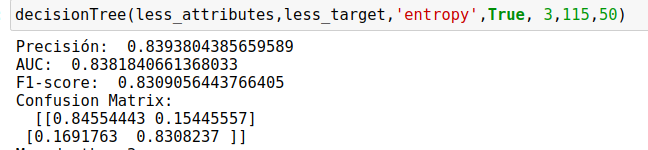
\includegraphics[width=1\linewidth]{img/image6}
	\caption{}
	\label{fig:image6}
\end{figure}

de manera que los resultados son algo mejores que en el caso en el que cambiamos solo la profundidad o el mínimo número de ejemplos en un nodo para que la división sea posible, pero un poco peores que si modificamos únicamente el mínimo número de ejemplos en los nodos hoja. Esto puede ser porque se compensan los resultados de los tres casos. 

Por la tanto, podemos concluir que los mejores resultados en el caso de los árboles de decisión se obtienen para la medida de Entropía y \mintinline{python}{min_samples_leaf=50}, quedando los otros valores por defecto. 

\subsection{Random Forest}

Este algoritmo combina varios árboles de decisión, de manera que la mayoría de los parámetros son comunes a estos, estudiados arriba. Así pues, para estos parámetros comunes consideraremos los valores que ya hemos visto que nos dan los mejores resultados, esto es, medida de Entropía y \mintinline{python}{min_samples_leaf=50}. 

Una vez fijados estos parámetros, lo más importante a configurar es el número de árboles con los que trabajamos, pues esto tiene un gran efecto en la reducción del overfitting, de manera que de cuantos más árboles dispongamos más se reducirá el overfitting que tendríamos uno solo de los árboles. Sin embargo, más árboles no siempre es mejor, pues también hay que tener en cuenta el coste computacional del aprendizaje de cada uno de ellos (cuantos más árboles, más coste). Además un número de árboles muy elevado también puede empeorar los resultados, como veremos. Buscamos pues, el número de árboles que nos da mejores resultados. 

\begin{table}[htbp]
	\caption{}
	\centerline{
		\begin{tabular}{|c|r|r|r|r|r|r|}
			\hline
			\multicolumn{1}{|l|}{num trees} & \multicolumn{1}{c|}{\textbf{10}} & \multicolumn{1}{c|}{\textbf{50}} & \multicolumn{1}{c|}{\textbf{100}} & \multicolumn{1}{c|}{\textbf{150}} & \multicolumn{1}{c|}{\textbf{200}} & \multicolumn{1}{c|}{\textbf{300}} \\ \hline
			Accuracy & 0.83702053602 & 0.83938739993 & 0.84174730247 & 0.84411416637 & 0.84175426383 & 0.84057779324 \\ \hline
			AUC & 0.835214200722 & 0.837846321776 & 0.840035415474 & 0.842474192824 & 0.839908833347 & 0.838944107535 \\ \hline
			F1-score & 0.822478563515 & 0.82699200934 & 0.829080958881 & 0.830187153504 & 0.826978704443 & 0.82483678308 \\ \hline
	\end{tabular}}
	\label{}
\end{table}

Tenemos que para un número pequeño de árboles los resultados son peores, pues se sigue produciendo overfitting, y cuando este número aumenta mejoran las predicciones. Para un número elevado de árboles, sin embargo, los resultados empeoran un poco, de manera que, de los valores estudiados, el que mejor resultados nos da es un número de 150 árboles. 

Cabe observar que, sin embargo, las métricas de evaluación nos dan valores más bajos aquí que para el mejor de los casos cuando teníamos un solo árbol. Esto no es así en la mayoría de los casos, pero aquí ocurre. Estudiaremos este fenómeno más adelante, en el apartado de \textbf{Análisis de Resultados}. 

Veamos ahora el efecto que tenemos si desactivamos el \textbf{bootstrapping}:

\begin{figure}[H]
	\centering
	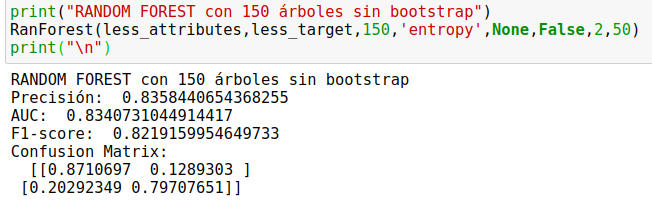
\includegraphics[width=1\linewidth]{img/img7}
	\caption{}
	\label{fig:img7}
\end{figure}

Esto es, los resultados son peores que si está activado. El bootstrapping añade aleatoriedad a los árboles, de manera que estos parten de ejemplos de entrenamiento diferentes, y si este está desactivado todos los árboles usarán los mismos datos. Esto hace que la correlación entre los distintos árboles aumente, con lo que el error asociado a cada árbol será parecido en todos y no se paliará el error medio, lo cual es el objetivo del algoritmo que estamos considerando. Es lógico, por tanto, que los resultados sean peores si desactivamos el bootstrapping.

Resumiendo, para \textbf{Random Forest} hemos obtenido los mejores resultados con 150 árboles (todos configurados como vimos en el apartado anterior) y el bootstrapping activado. 

\subsection{Redes Neuronales}

En una \textbf{Red Neuronal} los párametros más importantes a configurar son el \textit{learning rate}, el número de iteraciones, el número de \textit{hidden layers} y el número de nodos en cada \textit{hidden layer}.

Para un learning rate muy alto, el aprendizaje es más rápido, pero cabe el riesgo de caer en mínimos locales y que el algoritmo no converja hacia el mínimo global (de la función coste que se intenta optimizar en una red neuronal). Por el contrario, si el learning rate es muy bajo, la red neuronal puede tardar mucho tiempo en aprender y el coste computacional es, por tanto, más alto. 

Por otro lado, el número de capas ocultas y el número de nodos en cada una, es crucial para un correcto aprendizaje. Si la red es muy compleja, es decir, está formada por muchas capas ocultas y muchos nodos, es muy probable que se produzca sobreajuste a los datos de entrenamiento, con lo que el rendimiento de la red sería malo. Por otro lado, si tenemos una red muy sencilla, sin un número suficiente de capas ocultas o nodos, la red no aprendería todas las características necesarias para clasificar correctamente las instancias. Así pues, es importante encontrar unos valores adecuados para estos parámetros.  

El número de iteraciones también influye en el aprendizaje, pues para un número pequeño puede ser que no haya convergencia al mínimo global y las clasificaciones sean incorrectas, mientras que un número muy alto conlleva un coste computacional más elevado. 

Para disminuir el overfitting en redes neuronales se usa la regularización. El parámetro que nos proporciona \mintinline{python}{MLPClassifier} para controlar la regularización es \mintinline{python}{alpha}, de modo que valores mayores de alpha aumentan el efecto de la regularización, y por tanto disminuyendo el overfitting. 

 
Esta vez vamos a usar la funcionalidad  \mintinline{python}{GridSearchCV} de \mintinline{python}{sklearn.model_selection}, que se encarga de buscar los mejores valores para cada parámetro dentro de un espacio de parámetros proporcionado. 


A la función de activación le dejamos el valor por defecto, esto es, consideramos la función \textit{relu}, pues es la que funciona mejor en la mayoría de los casos. Para el método de optimización de los pesos, parámetro \mintinline{python}{solver}, nos quedamos con \textit{L-BFGS}, pues, según la documentación de \mintinline{python}{MLPClassifier}, en conjuntos de datos pequeños, como es nuestro caso, este optimizador funciona mejor y además hace que la convergencia sea más rápida. Al seleccionar este valor para \mintinline{python}{solver}, nos podemos olvidar del learning rate, pues este algoritmo no lo usa. Deberíamos considerar el learning rate solo si trabajásemos con Adam o Stochastic Gradient Descent, que no es nuestro caso. Así pues, a \mintinline{python}{learning_rate_init} le dejamos el valor por defecto que es $0.001$ y a \mintinline{python}{learning_rate} también, esto es, lo dejamos constante. 
 
Para el número de capas ocultas y número de nodos en cada una, influencia de la regularización (parámetro alpha) y número de iteraciones, vamos a empezar probando algunos valores dispersos. 

El código quedaría como sigue:
 
\begin{minted}{python}
from sklearn.model_selection import GridSearchCV

mlp=MLPClassifier()
parameter_space = {
	'hidden_layer_sizes': [(100,),(100,50),(200,100,50),(10,20,10)],
	'solver': ['lbfgs'],
	'alpha': [0.001, 0.05,0.01],
	'max_iter':[1000,10000],
}

clf=GridSearchCV(mlp, parameter_space, n_jobs=-1, cv=5)
clf.fit(less_attributes,less_target)
print('Mejores parámetros: ', clf.best_params_)
 \end{minted}
 
 
 del que obtenemos la siguiente salida:
 
  \begin{minted}{python}
 Mejores parámetros:  {'alpha': 0.001, 'hidden_layer_sizes': (10, 20, 10),
  'max_iter': 10000, 'solver': 'lbfgs'}
 
  \end{minted}
  
  Corremos entonces la red neuronal con estos parámetros y observamos los resultados. Además, vamos a probar a aumentar el número de iteraciones y comprobar si hay mejora. 
  
  \begin{table}[htbp]
  	\caption{}
  	\centerline{
  		\begin{tabular}{|c|r|r|}
  			\hline
  			max\_iter= & \multicolumn{1}{c|}{\textbf{10000}} & \multicolumn{1}{c|}{\textbf{100000}} \\ \hline
  			Accuracy & 0.842930734423947 & 0.842930734423947 \\ \hline
  			AUC & 0.84242559213514 & 0.84242559213514 \\ \hline
  			F1-score & 0.832818429754108 & 0.832818429754108 \\ \hline
  	\end{tabular}}
  	\label{}
  \end{table}
  
  y los resultados son exactamente iguales, con lo que no merece la pena aumentar el número de iteraciones y a partir de ahora trabajamos con \mintinline{python}{max_iter=10000}.
  
  Probamos ahora con otros valores para las capas ocultas. En concreto, tomamos
  
  \begin{minted}{python}
 	parameter_space = {
	 	'hidden_layer_sizes': [(25,50,25),(10,20,10),(5,10,5),(10,20)],
	 	'solver': ['lbfgs'],
	 	'alpha': [0.001, 0.05,0.01],
	 	'max_iter':[10000],
 	}
  \end{minted}
  
  y obtenemos 
  
  \begin{minted}{python}
  
  Mejores parámetros:  {'alpha': 0.05, 'hidden_layer_sizes': (25, 50, 25), 
  'max_iter': 10000, 'solver': 'lbfgs'}
  
  \end{minted}
 
 de manera que 
 
 \begin{table}[htbp]
 	\caption{}
 	\centerline{
 		\begin{tabular}{|c|r|}
 			\hline
 			Accuracy & 0.84292377305952 \\ \hline
 			AUC & 0.842536966930775 \\ \hline
 			F1-score & 0.833420386887948 \\ \hline
 	\end{tabular}}
 	\label{}
 \end{table}
 
 y efectivamente los resultados han mejorado ligeramente con respecto al caso anterior (excepto la precisión que ha bajado un poco).
 
Analizamos ahora alguna otra configuración de las capas ocultas y distintos valores de alpha: 

\begin{minted}{python}
parameter_space = {
	'hidden_layer_sizes': [(25,50,25),(50,100,50),(100,150,100),(100,50,25),(25,25,25)],
	'solver': ['lbfgs'],
	'alpha': [0.0001,0.001, 0.05,0.1,0.25,0.08],
	'max_iter':[10000],
}
\end{minted}

obteniendo

\begin{minted}{python}
	Mejores parámetros:  {'alpha': 0.25, 'hidden_layer_sizes': (25, 25, 25), 
	'max_iter': 10000, 'solver': 'lbfgs'}
\end{minted}

pero aquí los resultados empeoran un poco:

\begin{table}[H]
	\caption{}
	\centerline{
		\begin{tabular}{|c|r|}
			\hline
			Accuracy & 0.8346954403063 \\ \hline
			AUC & 0.834544834343587 \\ \hline
			F1-score & 0.823938289870037 \\ \hline
	\end{tabular}}
	\label{}
\end{table}


Por último, probamos a mano con algunas otras configuraciones.

Los resultados obtenidos para los distintos valores de los parámetros considerados han sido los siguientes:

\begin{table}[htbp]
	\caption{}
	\centerline{
		\begin{tabular}{|c|r|r|r|l|}
			\hline
			Capas ocultas & \multicolumn{1}{c|}{\textbf{(10,20,10)}} & \multicolumn{1}{c|}{\textbf{(25,50,25)}} & \multicolumn{1}{c|}{\textbf{(25,25,25)}} &  \\ \hline
			alpha & \multicolumn{1}{c|}{\textbf{0.001}} & \multicolumn{1}{c|}{\textbf{0.05}} & \multicolumn{1}{c|}{\textbf{0.25}} &  \\ \hline
			Accuracy & 0.842930734423 & 0.84292377305 & 0.8346954403 &  \\ \hline
			AUC & 0.84242559213 & 0.84253696693 & 0.834544834343 &  \\ \hline
			F1-score & 0.832818429754 & 0.833420386887 & 0.82393828987 &  \\ \hline
			\multicolumn{1}{|l|}{} & \multicolumn{1}{l|}{} & \multicolumn{1}{l|}{} & \multicolumn{1}{l|}{} &  \\ \hline
			\multicolumn{1}{|l|}{} & \multicolumn{1}{l|}{} & \multicolumn{1}{l|}{} & \multicolumn{1}{l|}{} &  \\ \hline
			Capas ocultas & \multicolumn{1}{c|}{\textbf{(10,20,10)}} & \multicolumn{1}{c|}{\textbf{(100,50,25)}} & \multicolumn{1}{c|}{\textbf{(100,50,25)}} & \multicolumn{1}{c|}{\textbf{(25,25,25)}} \\ \hline
			alpha & \multicolumn{1}{c|}{\textbf{0.05}} & \multicolumn{1}{c|}{\textbf{0.08}} & \multicolumn{1}{c|}{\textbf{0.05}} & \multicolumn{1}{c|}{\textbf{0.001}} \\ \hline
			Accuracy & 0.83586494953 & 0.84290985033 & 0.835837104072 & \multicolumn{1}{r|}{0.840556909154} \\ \hline
			AUC & 0.8358058678916 & 0.84169288182 & 0.8343120992354 & \multicolumn{1}{r|}{0.8396366598416} \\ \hline
			F1-score & 0.8252829003886 & 0.831105442869 & 0.821845353228 & \multicolumn{1}{r|}{0.8283231073911} \\ \hline
	\end{tabular}}
	\label{}
\end{table}

Para todas las configuraciones de parámetros estudiadas, los resultados son bastante parecidos, obteniendo los que son un poco mejores en dos casos:

\begin{enumerate}
	\item Para una configuración (10,20,10) de las capas ocultas (esto es, 10 nodos en la primera capa, 20 en la segunda y 10 en la tercera) y un valor de alpha de 0.001 (poca influencia de la regularización).
	\item Capas ocultas de la forma (25,50,25) (tres capas con 25 nodos en la primera y tercera y 50 en la segunda) y parámetro de regularización con un valor de 0.05 (mayor influencia de la regularización). Puesto que aquí la red es algo más compleja, pues tenemos un mayor número de nodos, es lógico que haya que aumentar la influencia de la regularización, ya que el sobreajuste en esta red es más influyente.
	
\end{enumerate}

De las dos configuraciones, la que nos ofrece valores ligeramente mejores para el AUC y F1-score es la segunda, y, puesto que estas medidas son más importantes en nuestro estudio que la precisión, consideraremos a partir de ahora la segunda de las configuraciones como la mejor para este modelo. A cambio de mejores resultados nos encontramos con una red más compleja, por lo que, si la complejidad es un problema, elegiríamos la primera de las configuraciones enumeradas arriba.



\newpage
\section{Resultados obtenidos}

Para el entrenamiento de los modelos y estudio de los resultados usaremos la siguiente función, que implementa la validación cruzada con 5 particiones y muestra por pantalla los resultados de algunas métricas de evaluación tras entrenar el modelo proporcionado como parámetro y clasificar los datos de test.


\begin{minted}{python}
'''
Función genérica para resolver el problema de clasificación.
Muestra por pantalla los resultados de las métricas de 
evaluación tras entrenar el modelo y predecir las clases sobre el 
conjunto de datos de test

X -> Conjunto de atributos que se usarán para predecir la clases
Y -> Etiquetas de las clases
clf -> Clasificador que se usará para resolver el problema 

No devuelve nada 

'''

def clasificacion(X,Y,clf):
	kf=KFold(n_splits=5,shuffle=True,random_state=100)
	
	f1,auc,accuracy=0,0,0
	cm=np.zeros((2,2))
	
	for train_index, test_index in kf.split(X):
	x_train, x_test = X.iloc[train_index], X.iloc[test_index]
	y_train, y_test = Y.iloc[train_index], Y.iloc[test_index]
	
	clf.fit(x_train, y_train)
	pred=clf.predict(x_test)
	
	auc=auc+roc_auc_score(y_test,pred)
	
	accuracy=accuracy+accuracy_score(y_test, pred, normalize=True)
	f1=f1+f1_score(y_test, pred)
	cm=cm+confusion_matrix(y_test,pred,normalize='true')

print("Precisión: ", accuracy/5)
print("AUC: ", auc/5)
print("F1-score: ",f1/5)
print("Confusion Matrix:\n ", cm/5)
\end{minted}

En concreto, consideramos las siguientes medidas de evaluación:
\begin{itemize}
	\item \textbf{Precisión (accuracy)}, que nos indica el porcentaje de casos en los que el modelo acierta en sus predicciones. En el caso de clases que no están balanceadas, esta medida no es muy efectiva y conviene considerar otro tipo de métricas. Este no es un gran problema en nuestro caso. Aún así estudiamos también:
	\item \textbf{AUC}, devuelve el área bajo la curva ROC, de manera que cuanto mayor sea este valor mejor es el clasificador. Esta medida es robusta frente a las clases imbalanceadas, por lo que es más representativa de la bondad del clasificador.
	\item \textbf{F1-score}, que es la media ármonica entre PPV (predicciones positivas correctas entre el número total de predicciones positivas) y TPR (predicciones positivas correctas entre entre el número total de postivos reales). Esta medida penaliza más los errores al clasificar ejemplos positivos (cancer maligno) que al clasificar ejemplos negativos (cancer benigno). Por lo tanto, es una medida con más importancia en nuestro estudio, como ya hemos comentado anteriormente, pues es más grave cometer errores al determinar un cancer maligno que un cancer benigno.
	\item \textbf{Matriz de confusión}
\end{itemize}

Como se puede observar en el código, consideramos la media de los resultados obtenidos de estas medidas en cada partición de la validación cruzada, y tomamos esas medias como los resultados para el clasificador de las métricas correspondientes. 

Pasamos entonces a ver los resultados obtenidos de estas métricas para los distintos clasificadores estudiados. Para cada uno mostramos los resultados para la mejor configuración de los parámetros, determinada en el apartado anterior. 
\subsection{Linear SVC}

Este modelo lo hemos estudiado haciendo uso de \mintinline{python}{svm.LinearSVC} de \mintinline{python}{sklearn}, así como de la función \mintinline{python}{clasificacion} cuyo código ya hemos visto. Implementamos así la siguiente función, de modo que los parámetros considerados coindicen con los de \mintinline{python}{svm.LinearSVC} del mismo nombre, excepto X e Y:

\begin{minted}{python}
from sklearn.svm import LinearSVC

def svm(X,Y,C=1.0,class_weight=None,max_iter=1000):
	clf=LinearSVC(C=C,class_weight=class_weight,random_state=10,max_iter=max_iter)
	clasificacion(X,Y,clf)
\end{minted}

Los parámetros de este clasificador no han sido estudiados en el apartado anterior, con lo que mostramos aquí los resultados mejores obtenidos tras ejecutarlo con diversos parámetros:

\begin{table}[htbp]
	\caption{}
	\centerline{
		\begin{tabular}{|c|r|}
			\hline
			\textbf{Accuracy} & 0.831152105812739 \\ \hline
			\textbf{AUC} & 0.831423981332614 \\ \hline
			\textbf{F1-score} & 0.826288144700667 \\ \hline
	\end{tabular}}
	\label{}
\end{table}


\begin{table}[htbp]
	\caption{Matriz de confusión}
	\centerline{
		\begin{tabular}{|l|l|r|l|}
			\hline
			\multicolumn{ 1}{|l|}{} &  & \multicolumn{1}{c|}{\textbf{Predicción}} &  \\ \cline{ 2- 4}
			\multicolumn{ 1}{|l|}{} &  & \multicolumn{1}{l|}{\textit{Positivo (maligno)}} & \textit{Negativo (benigno)} \\ \cline{ 2- 4}
			\multicolumn{1}{|c|}{\textbf{Clase real}} & \textit{Positivo (maligno)} & 0.81710525 & \multicolumn{1}{r|}{0.18289475} \\ \hline
			& \textit{Negativo (benigno)} & 0.15425729 & \multicolumn{1}{r|}{0.84574271} \\ \hline
	\end{tabular}}
	\label{}
\end{table}

donde los parámetros que hemos considerado han sido \mintinline{python}{C=5} (parámetro de regularización), un número de iteraciones de 100000000 y pesos 'balanceados' para las clases.
\subsection{Vecinos más cercanos Knn}

Para implementar este modelo, usamos el clasificador \mintinline{python}{neighbors.KNeighborsClassifier} de \mintinline{python}{sklearn} y la función \mintinline{python}{clasificacion} mostrada arriba, de manera que el código quedaría como sigue:

\begin{minted}{python}
	from sklearn.neighbors import KNeighborsClassifier
	
	def Knn(X,Y,n_neighbors,weights,p,metric='minkowski'):
		clf=KNeighborsClassifier(n_neighbors=n_neighbors, 
		weights=weights, p=p,metric=metric)
		clasificacion(X,Y,clf)
\end{minted}

donde los parámetros que se le pasan a nuestra función coindicen con los parámetros del clasificador \mintinline{python}{KNeighborsClassifier}, excepto \textbf{X} e \textbf{Y} que son los datos, concretamente los atributos y las etiquetas respectivamente. 

Los mejores resultados obtenidos con él han sido los siguientes:

\begin{table}[htbp]
	\caption{}
	\centerline{
		\begin{tabular}{|c|r|}
			\hline
			\textbf{Accuracy} & 0.822937695788375 \\ \hline
			\textbf{AUC} & 0.821203748872583 \\ \hline
			\textbf{F1-score} & 0.803150545123026 \\ \hline
	\end{tabular}}
	\label{}
\end{table}

\begin{table}[htbp]
	\caption{Matriz de Confusión}
	\centerline{
		\begin{tabular}{|l|l|r|l|}
			\hline
			&  & \multicolumn{1}{c|}{\textbf{Predicción}} &  \\ \hline
			&  & \multicolumn{1}{l|}{\textit{Positivo (maligno)}} & \textit{Negativo (benigno)} \\ \hline
			\multicolumn{1}{|c|}{\textbf{Clase real}} & \textit{Positivo (maligno)} & 0.89519431 & \multicolumn{1}{r|}{0.10480569} \\ \hline
			& \textit{Negativo (benigno)} & 0.25278681 & \multicolumn{1}{r|}{0.74721319} \\ \hline
	\end{tabular}}
	\label{}
\end{table}
\subsection{Árboles de decisión}

En este caso usamos  \mintinline{python}{tree.DecisionTreeClassifier} de \mintinline{python}{sklearn} y la función \mintinline{python}{clasificacion}. Tenemos aquí una novedad con respecto a los casos anteriores, y es que además de los parámetros propios de \mintinline{python}{DecisionTreeClassifier} y el conjunto de datos (X e Y), añadimos dos nuevos a nuestra función que son \mintinline{python}{depth} y \mintinline{python}{plot}, ambos con valor \mintinline{python}{False} por defecto. Si activamos el primero (\mintinline{python}{depth=True}), además de las medidas de evaluación mencionadas hasta ahora, se muestran otras medidas de la complejidad del árbol, a saber, la profundidad del mismo, el número de hojas y el número de nodos. Por otro lado, si ponemos \mintinline{python}{plot=True}, se genera una imagen png con la representación gráfica del árbol aprendido. Así pues, el código sería el siguiente: 


\begin{minted}{python}
	from sklearn.tree import DecisionTreeClassifier,export_graphviz
	import graphviz
	
	def decisionTree(X,Y, criterion,depth=False,max_depth=None, 
	min_samples_split=2,min_samples_leaf=1,plot=False):
		clf=DecisionTreeClassifier(criterion=criterion,max_depth=max_depth,
		min_samples_split=min_samples_split,min_samples_leaf=min_samples_leaf,
		random_state=100)
		clasificacion(X,Y,clf)
		if depth:
			print("Max depth: ", clf.tree_.max_depth)
			print("Número de hojas: ", clf.get_n_leaves())
			print("Número de nodos: ", clf.tree_.node_count)
		if plot:
			dot_data = export_graphviz(clf, out_file=None,
			feature_names=X.columns, class_names=['benigno','maligno'],
			filled=True)
			graph = graphviz.Source(dot_data, format="png")
			graph.render('decision_tree') 
			graph
	
\end{minted}

Y los resultados para la configuración de parámetros ya estudiada son:

\begin{table}[H]
	\caption{}
	\centerline{
		\begin{tabular}{|c|r|r|r|}
			\hline
			\textbf{} & \multicolumn{1}{c|}{\textbf{max\_depth=3}} & \multicolumn{1}{c|}{\textbf{min\_samples\_split=115}} & \multicolumn{1}{c|}{\textbf{min\_samples\_leaf=50}} \\ \hline
			Accuracy & 0.837020536 & 0.832286808214 & 0.845297598329272 \\ \hline
			AUC & 0.83528944478 & 0.83164615740393 & 0.843296425687365 \\ \hline
			F1-score & 0.81878189759 & 0.81748160812375 & 0.834270875636609 \\ \hline
			max depth & 3 & 7 & 5 \\ \hline
			num hojas & 7 & 14 & 10 \\ \hline
			num nodos & 13 & 27 & 19 \\ \hline
	\end{tabular}}
	\label{}
\end{table}

de donde deducimos que los árboles menos complejos son para \mintinline{python}{max_depth=3} y \mintinline{python}{min_samples_leaf=50}, lo cual es lógico pues son los que nos dan mejores resultados ya que el overfitting en ellos es menor. 

Por otra parte, las matrices de confusión obtenidas en cada uno de los casos son:

\begin{table}[H]
	\caption{max depth=3}
	\centerline{
		\begin{tabular}{|l|l|r|l|}
			\hline
			\multicolumn{ 1}{|l|}{} &  & \multicolumn{1}{c|}{\textbf{Predicción}} &  \\ \cline{ 2- 4}
			\multicolumn{ 1}{|l|}{} &  & \multicolumn{1}{l|}{\textit{Positivo (maligno)}} & \textit{Negativo (benigno)} \\ \cline{ 2- 4}
			\multicolumn{1}{|c|}{\textbf{Clase real}} & \textit{Positivo (maligno)} & 0.89923105 & \multicolumn{1}{r|}{0.10076895} \\ \hline
			& \textit{Negativo (benigno)} & 0.22865216 & \multicolumn{1}{r|}{0.77134784} \\ \hline
	\end{tabular}}
	\label{}
\end{table}

\begin{table}[H]
	\caption{min samples split=115}
	\centerline{
		\begin{tabular}{|l|l|r|l|}
			\hline
			\multicolumn{ 1}{|l|}{} &  & \multicolumn{1}{c|}{\textbf{Predicción}} &  \\ \cline{ 2- 4}
			\multicolumn{ 1}{|l|}{} &  & \multicolumn{1}{l|}{\textit{Positivo (maligno)}} & \textit{Negativo (benigno)} \\ \cline{ 2- 4}
			\multicolumn{1}{|c|}{\textbf{Clase real}} & \textit{Positivo (maligno)} & 0.87694447 & \multicolumn{1}{r|}{0.12305553} \\ \hline
			& \textit{Negativo (benigno)} & 0.21365216 & \multicolumn{1}{r|}{0.78634784} \\ \hline
	\end{tabular}}
	\label{}
\end{table}

\begin{table}[H]
	\caption{min samples leaf=50}
	\centerline{
		\begin{tabular}{|l|l|r|l|}
			\hline
			\multicolumn{ 1}{|l|}{} &  & \multicolumn{1}{c|}{\textbf{Predicción}} &  \\ \cline{ 2- 4}
			\multicolumn{ 1}{|l|}{} &  & \multicolumn{1}{l|}{\textit{Positivo (maligno)}} & \textit{Negativo (benigno)} \\ \cline{ 2- 4}
			\multicolumn{1}{|c|}{\textbf{Clase real}} & \textit{Positivo (maligno)} & 0.86576915 & \multicolumn{1}{r|}{0.13423085} \\ \hline
			& \textit{Negativo (benigno)} & 0.1791763 & \multicolumn{1}{r|}{0.8208237} \\ \hline
	\end{tabular}}
	\label{}
\end{table}

\subsection{Random Forest}

Ahora trabajamos con \mintinline{python}{ensemble.RandomForestClassifier} y la función \mintinline{python}{clasificacion}, como siempre, de manera que tenemos el siguiente código:

\begin{minted}{python}
from sklearn.ensemble import RandomForestClassifier

def RanForest(X,Y,num_trees,criterion,max_depth=None, bootstrap=True,
min_samples_split=2,min_samples_leaf=1):
	clf=RandomForestClassifier(n_estimators=num_trees, criterion=criterion,
	max_depth=max_depth, bootstrap=bootstrap,min_samples_split=min_samples_split,
	min_samples_leaf=min_samples_leaf,random_state=100)
	clasificacion(X,Y,clf)
\end{minted}

donde de nuevo los parámetros coinciden con los de \mintinline{python}{RandomForestClassifier} menos X e Y.

Tenemos los resultados siguientes:

\begin{table}[htbp]
	\caption{}
	\centerline{
		\begin{tabular}{|c|r|}
			\hline
			\textbf{Accuracy} & 0.84411416637 \\ \hline
			\textbf{AUC} & 0.842474192824 \\ \hline
			\textbf{F1-score} & 0.830187153504 \\ \hline
	\end{tabular}}
	\label{}
\end{table}

\begin{table}[htbp]
	\caption{Matriz de Confusión}
	\centerline{
		\begin{tabular}{|l|l|r|l|}
			\hline
			& \multicolumn{ 1}{l|}{} & \multicolumn{1}{c|}{\textbf{Predicción}} &  \\ \cline{ 1- 1}\cline{ 3- 4}
			&  & \multicolumn{1}{l|}{\textit{Positivo (maligno)}} & \textit{Negativo (benigno)} \\ \hline
			\multicolumn{1}{|c|}{\textbf{Clase real}} & \textit{Positivo (maligno)} & 0.88274116 & \multicolumn{1}{r|}{0.11725884} \\ \hline
			& \textit{Negativo (benigno)} & 0.19779278 & \multicolumn{1}{r|}{0.80220722} \\ \hline
	\end{tabular}}
	\label{}
\end{table}

\subsection{Redes Neuronales}

Por último, veamos los mejores resultados que hemos obtenido para el caso de las redes neuronales, donde hemos hecho uso de \mintinline{python}{neural_network.MLPClassifier} y de nuevo la función \mintinline{python}{clasificacion}, con el código:
\begin{minted}{python}
from sklearn.neural_network import MLPClassifier

def NN(X,Y,hl_sizes,activation='relu',solver='adam',alpha=0.0001,learning_rate=0.001,
max_iter=200):
	clf=MLPClassifier(hidden_layer_sizes=hl_sizes, activation=activation, 
	solver=solver, alpha=alpha, learning_rate_init=learning_rate, 
	max_iter=max_iter,random_state=100)
	clasificacion(X,Y,clf)
\end{minted}

Y los resultados son los siguientes:

\begin{table}[htbp]
	\caption{}
	\centerline{
		\begin{tabular}{|c|r|}
			\hline
			\textbf{Accuracy} & 0.84292377305952 \\ \hline
			\textbf{AUC} & 0.842536966930775 \\ \hline
			\textbf{F1-score} & 0.833420386887948 \\ \hline
	\end{tabular}}
	\label{}
\end{table}

\begin{table}[H]
	\caption{Matriz de confusión}
	\centerline{
		\begin{tabular}{|l|l|r|l|}
			\hline
			\multicolumn{ 1}{|l|}{} &  & \multicolumn{1}{c|}{\textbf{Predicción}} &  \\ \cline{ 2- 4}
			&  & \multicolumn{1}{l|}{\textit{Positivo (maligno)}} & \textit{Negativo (benigno)} \\ \hline
			\multicolumn{1}{|c|}{\textbf{Clase real}} & \textit{Positivo (maligno)} & 0.85835406 & \multicolumn{1}{r|}{0.14164594} \\ \hline
			& \textit{Negativo (benigno)} & 0.17328013 & \multicolumn{1}{r|}{0.82671987} \\ \hline
	\end{tabular}}
	\label{}
\end{table}

En cuanto a la complejidad, ya vimos que en la mejor configuración la red está formada por 100 ($25+50+25$) nodos intermedios, lo cual indica que este modelo es bastante complejo, en comparación con los árboles de decisión, en los que, en los mejores casos, el valor más alto del número de nodos era de 27.



\newpage
\section{Análisis de resultados}

Comparamos ahora los resultados para los distintos clasificadores, analizando cuales son mejores y peores y las razones de ello. 

Empezamos viendo los resultados de cada uno en las siguientes tablas, considerando como siempre la mejor configuración de parámetros ya determinada:

\begin{table}[htbp]
	\caption{}
	\centerline{
		\begin{tabular}{|c|r|r|r|r|r|}
			\hline
			\multicolumn{1}{|l|}{} & \multicolumn{1}{c|}{\textbf{Linear SVC}} & \multicolumn{1}{c|}{\textbf{Knn}} & \multicolumn{1}{c|}{\textbf{Árbol de decisión}} & \multicolumn{1}{c|}{\textbf{Random Forest }} & \multicolumn{1}{c|}{\textbf{Red Neuronal}} \\ \hline
			Accuracy & 0.831152105812 & 0.822937695788 & 0.845297598329 & 0.84411416637 & 0.84292377305 \\ \hline
			AUC & 0.831423981332 & 0.821203748872 & 0.843296425687 & 0.842474192824 & 0.84253696693 \\ \hline
			F1-score & 0.8262881447 & 0.803150545123 & 0.834270875636 & 0.830187153504 & 0.83342038688 \\ \hline
	\end{tabular}}
	\label{}
\end{table}
 
Podemos observar que los mejores resultados se obtienen para los árboles de decisión y el Random Forest, siendo los primeros algo mejores, seguidos por las redes neuronales.

\begin{itemize}
 \item Los \underline{árboles de decisión} son un algoritmo bastante eficiente que proporciona buenos resultados, como podemos comprobar, además de que es robusto a los datos con ruido, trabaja bien con variables categóricas y es capaz de manejar adecuadamente los atributos irrelevantes que proporcionan poca información. Además de todo esto es un modelo de caja blanca, es decir, el resultado del entrenamiento es fácilmente interpretable y su costo computacional es muy bajo. Sin embargo, son bastante susceptibles al sobreaprendizaje, problema que en nuestro caso hemos tratado ajustando adecuadamente los parámetros para que el árbol no crezca indefinidamente. Por otro lado no tratan bien los outliers ni los atributos de tipo continuo y no son capaces de aprender conceptos demasiado complejos. 
 
 \item Por su parte, \underline{Random Forest} intenta disminuir el sobreaprendizaje de un árbol de decisión individual, considerando varios árboles por separado. Así, en general, los resultados de este algoritmo suelen ser más precisos y robustos que los de un árbol de decisión. No obstante, no funciona bien si los árboles o, más concretamente, sus predicciones, están correladas. Además, cuando el 'bosque' crece también lo hace el coste computacional y, por otra parte, perdemos la interpretabilidad con la que tan gratamente cóntabamos en los árboles de decisión.
\end{itemize}

Aunque generalmente el algoritmo de Random Forest debería dar mejores resultados que un único árbol de decisión, aquí ocurre lo contrario. Aún siendo mínima la diferencia, cabe observar en la tabla que las medidas en el mejor de los casos de un árbol de decisión son mejores que en Random Forest. Esto ya lo comentamos cuando ajustamos los parámetros de este algoritmo. Una explicación lógica por la que esto sucede podría ser que, como en Random Forest cada árbol individual trabaja con menos datos y menos atributos (debido al bagging), aumenta el underfitting en cada árbol, y los resultados proporcionados por cada uno de ellos tienen más errores, de manera que la predicción general también es peor. También podría ser un indicador de que el sobreajuste no es un problema tan grande tras configurar adecuadamente un árbol de decisión individualmente, pues al intentar disminuir el overfitting con \textbf{Random Forest} los resultados no han mejorado en absoluto.  

El siguiente modelo que nos da mejores predicciones son las redes neuronales.
\begin{itemize}
	\item Las \underline{Redes Neuronales} es generalmente de los modelos que proporcionan mejores predicciones  en los problemas de clasificación y son más robustas que los árboles de decisión. Además, al contrario que los árboles de decisión, tratan bien con los outliers, además de con el ruido. Son capaces de aprender conceptos muy complejos, que los árboles de decisión no podrían aprender. Sin embargo, para poder ser bien entrenadas, las redes neuronales necesitan disponer de gran cantidad de datos, además de largo tiempo de aprendizaje. Puede ocurrir que la función de coste que se busca optimizar caiga en mínimos locales, y por tanto, la red no sería entrenada correctamente. Por otro lado, es muy difícil o prácticamente imposible interpretarlas, se trata de un modelo de caja negra. 
	
	Cuando la red es muy compleja, puede incurrir en sobreaprendizaje, al igual que los árboles de decisión, y dispone de numerosos hiperparámetros que hay que tunear, lo cual no es tarea sencilla. 
\end{itemize}

Un motivo por el que este modelo no nos da resultados tan buenos en nuestro caso es porque disponemos de pocos datos y ya hemos dicho que las redes neuronales no trabajan bien con conjuntos de datos pequeños. Por otra parte, sus hiperparámetros han de ser exhaustivamente ajustados, lo cual no hemos llevado acabo aquí, de manera que es probable que para otros parámetros los resultados sean mejores incluso que los del árbol de decisión. Otro motivo por el que obtenemos resultados más bajos puede ser el sobreajuste, pues una red  muy compleja es propensa al sobreaprendizaje. Mientras que en los árboles de decisión hemos intentado lidiar con este más en profundidad, en las redes neuronales no nos hemos parado tanto, con lo que puede ser que haya que reducir el soberajuste aún más. En resumen, si dispusiéramos de más datos y más tiempo para entrenar con más detalle la red neuronal, puede que esta nos hubiera dado mejores predicciones. Pero dadas las circusntancias, puesto que nuestro conjunto de datos es pequeño y no aspiramos a resultados mucho mejores, los proporcionados por el árbol de decisión son suficientes. Es más, con el árbol de decisión tenemos una interpretabilidad del modelo con la que no contamos en las redes neuronales, además de que es mucho menos complejo, como ya vimos en el apartado de \textbf{Resultados obtenidos}.

Los dos modelos con los que hemos obtenido los peores resultados han sido los vecinos más cercanos y las máquinas lineales de soporte vectorial, aunque estas últimas proporcionan datos algo mejores.

\begin{itemize}
	\item El algoritmo del \underline{vecino} (o vecinos en nuestro caso) \underline{más cercano} es uno de los más sencillos. Es robusto frente al ruido para valores adecuados de \textit{k}, esto es, para valores pequeños se deja llevar por el ruido y para valores demasiado grandes también. Al contrario que las redes neuronales, tiene pocos hiperparámetros que configurar, siendo \textit{k} el más importante, y el tiempo requerido para el entrenamiento es nulo. Sin embargo, consume mucha memoria, puesto que requiere que todos los datos permanezcan almacenados e implica alto coste computacional, ya que la clasificación tiene lugar en tiempo de ejecución y, si el conjunto de datos es grande, necesita bastante tiempo para calcular todas las distancias entre los datos. Además, puede dejarse llevar por atributos poco representativos, es decir, atributos irrelevantes, lo cual no ocurre con los árboles de decisión. También es propenso al sobreajuste si no se configura adecuadamente el parámetro \textit{k}, y es bastante sensible a los outliers.  

	\item Las \underline{máquinas de soporte vectorial lineales} (LinearSVC) son más eficientes en espacios multidimensionales (los datos tienen multiples atributos), incluso si el número de dimensiones es mayor que el número de ejemplos (no es nuestro caso). Necesitan menos datos de entrenamiento que las redes neuronales para dar buenos resultados. Requieren que los datos sean linealmente separables, lo cual no era necesario en el resto de clasificadores estudiados. Como sólo necesita los vectores de soporte para realizar la predicción, consume poca memoria, no como el algoritmo \textit{K-nn}. Por otra parte, puede tratar con los outliers (mejor que K-nn), así como con el sobreaprendizaje, ajustando adecuadamente la \textit{constante de margen suave} (C), el cual es casi el único parámetro a optimizar (en contraste con las redes neuronales que tienen muchos hiperparámetros).
\end{itemize}

Podemos deducir entonces que este último modelo nos da resultados algo peores que las redes neuronales y los árboles de decisión por requerir la separación lineal completa de lo datos, lo cual no sabemos con certeza que se de en nuestro caso. No obstante, los resultados no son tan bajos, de modo que es probable que nuestros datos se puedan separar linealmente, aunque no por completo. Además, no hemos optimizado con detenimiento el parámetro C, con lo que es probable que aún se puedan mejorar los resultados, configurando mejor este parámetro para reducir el sobreaprendizaje y prescindir de los outliers. 

Sin embargo, LinearSVC nos ofrece mejores predicciones que K-nn. Aunque K-nn es de los algoritmos más sencillos, presenta los peores resultados, probablemente porque considere atributos irrelevantes en la clasificación, se deje llevar por los outliers o porque haya sobreajuste, el cual no podamos reducir ni incluso configurando el valor de k. Además, su coste computacional es muy elevado, como hemos mencionado. Por lo tanto, podríamos decir que no es un modelo muy bondadoso. 


Los resultados con estos dos últimos clasificadores tampoco son fácilmente interpretables, como ocurre con los árboles de decisión, lo cual es otra desventaja de ambos. 


En conclusión, tras analizar los resultados obtenidos y estudiar las ventajas y desventajas de cada uno de los modelos, podemos decir que el clasificador que mejor se adapta a nuestras circunstancias es el árbol de decisión, tanto porque nos ha proporcionado los mejores resultados, como por su interpretabilidad y menor coste computacional. En el lado opuesto tenemos el algoritmo del vecino más cercano con su alto coste computacional y alto consumo de memoria, que, a pesar de su sencillez, ofrece los peores resultados.

\newpage
\section{Interpretación de resultados}

En este apartado intentamos extraer conclusiones sobre los factores más importantes que determinan que el tumor sea maligno o benigno. Puesto que el único algoritmo que proporciona resultados interpretables de los estudiados son los árboles de decisión, partiremos de estos para llegar a dichas conclusiones. Para ello, visualizamos el árbol de decisión resultante del entrenamiento para la configuración de parámetros con los que obtuvimos mejores resultados:

\begin{figure}[H]
	\centering
	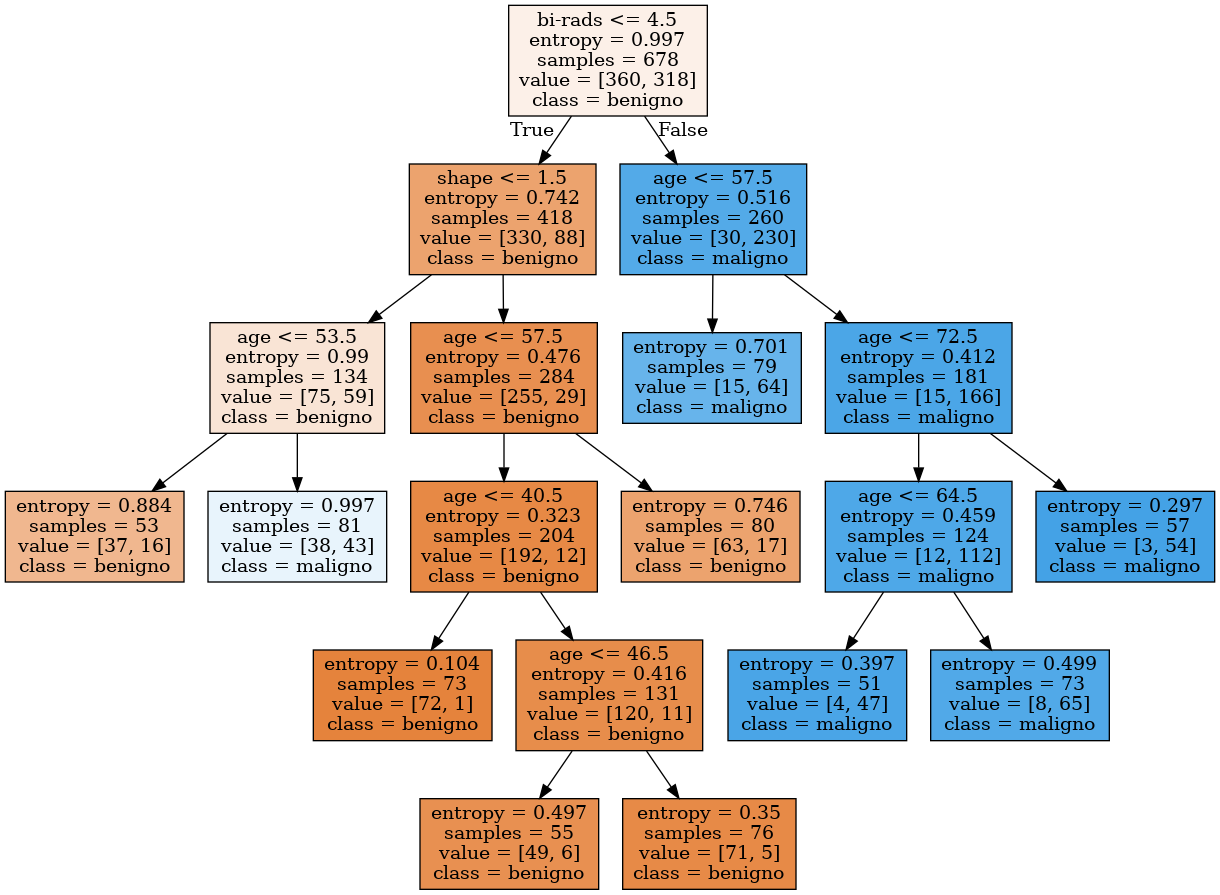
\includegraphics[width=1.1\linewidth]{img/decision_tree}
	\caption{}
	\label{fig:decisiontree}
\end{figure}

Puesto que en el nodo raíz el atributo de test que se escoge es el código BI-RADS, es claro que este es el que proporciona mayor ganancia en información y es, por tanto, el atributo que mejor determina la pertenencia a una clase u otra. Siguiendo a este, nos encontramos con el la edad y la forma de la masa anormal, de manera que estos dos también influyen en la clase a la que pertenece una instancia en gran medida, pues la ganancian de información asociada a los mismos también es elevada. En el resto de nodos, el único atributo considerado es la edad, lo cual reafirma la idea de que este atributo es importante en la clasificación. El resto de atributos de los que disponemos, el margen y la densidad de la masa, no se tienen en cuenta en este árbol, de modo que ambos tienen menos influencia en la pertenencia a una determinada clase. Sin embargo, esto no indica que no aporten información que pueda ser útil en algunos casos, solo que dicha información es menos relevante. En otros clasificadores puede ocurrir que dichos atributos sí tengan algún efecto. Por ejemplo, cuando en el preprocesamiento eliminamos el atributo del margen, vimos que los resultados para todos los clasificadores empeoraban un poco, aunque no excesivamente, por lo que se trata de una variable que aporta información para mejorar la clasificación, pero no es información imprescindible para predecir la clase. 

Por otro lado, si consideramos el árbol más simple que nos dio buenos resultados
\begin{figure}[H]
	\centering
	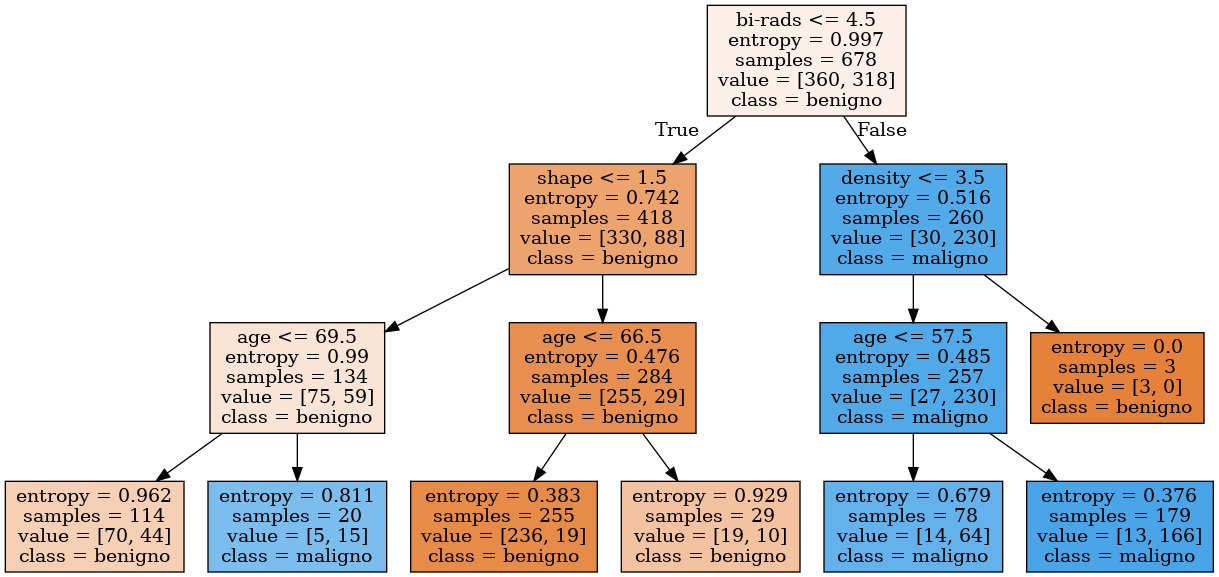
\includegraphics[width=1.1\linewidth]{img/decision_tree2}
	\caption{}
	\label{fig:decisiontree2}
\end{figure}


observamos que aquí sí aparece la densidad de la masa pero sigue sin aparecer el margen, con lo que tenemos más motivos para asegurar que este último no es tan importante como los demás. Además, el código BI-RADS vuelve a aparecer en la raíz del árbol, así que podemos reafirmar que se trata el atributo más importante. En el siguiente nivel nos volvemos a encontrar con la forma, pero ahora en vez de la edad tenemos  la densidad. En el resto de nodos solo se considera la edad como atributo de test.


Veamos ahora el camino que siguen algunos ejemplos aleatorios en los árboles de decisión. Consideramos para ello los siguientes datos de pacientes extraídos del conjunto de datos de partida:

\begin{enumerate}
	\item Valores de los atributos en orden: 4.0, 60.0, 3, 1.0, 2.0 Etiqueta: 0\\
	Árbol 1:\\
	 $4<4.5$ $\rightarrow$ izquierda\\
			  $ 3>1.5 $ $\rightarrow$ derecha\\
			  $ 60>57.5 $ $\rightarrow$ derecha\\
			  Y llegamos a la hoja, clasificando esta instancia como tumor benigno $\rightarrow$ \textbf{Correcto}
	\item Valores de los atributos en orden: 0.0, 71.0, 0, 4.0, 3.0	Etiqueta: 1\\
	Árbol 2:\\
	 $0.0 < 4.5$ $\rightarrow$ izquierda\\
			$ 0<1.5 $ $\rightarrow$ izquierda\\
			$ 71>95.5 $ $\rightarrow$ derecha\\
			Clasificación: maligno $\rightarrow$ \textbf{Correcto}
	\item Valores de los atributos en orden: 4.0, 70.0,	4, 1.0, 1.0	Etiqueta: 0\\
	Árbol 1:\\
		$ 4<4.5 $ $\rightarrow$ izquierda\\
		$ 4>1.5 $ $\rightarrow$ derecha\\
		$ 70>57.5 $ $\rightarrow$ derecha\\
		Clasificación: benigno $\rightarrow$ \textbf{Correcto}
		
	\item Valores de los atributos en orden: 5.0, 58.0,	0, 5.0, 3.0, 1 Etiqueta: 1\\
	Árbol 1:\\
	 $ 5>4.5 $ $\rightarrow$ derecha\\
	 $ 58<57.5 $ $\rightarrow$ izquierda\\
	 Clasificación: maligno $\rightarrow$ \textbf{Correcto}
	 
	 \item Valores de los atributos en orden: 5.0, 40.0, 1,	2.0, 3.0	 Etiqueta: 1\\
	 Árbol 2:\\
	 $ 5>4.5 $ $\rightarrow$ derecha\\
	 $ 3<3.5 $ $\rightarrow$ izquierda\\
	 $ 40<57.5 $ $\rightarrow$ izquierda \\
	 Clasificación: maligno $\rightarrow$ \textbf{Correcto}
	 
\end{enumerate}

Así, hemos conseguido clasificar los ejemplos aleatorios correctamente de manera sencilla, simplemente siguiendo las reglas del árbol. En ninguno de los casos hemos necesitado el valor del margen de la masa en el paciente, y, sin embargo, las predicciones han sido correctas. Además, solo hemos considerado el valor de dos o tres atributos a lo sumo, estando entre ellos siempre presente el código BI-RADS, de manera que no son todos necesarios para llevar a cabo una correcta clasificación una vez aprendido el árbol. 

Podemos concluir entonces que el atributo que más influye en la determinación de la clase es el código BI-RADS, seguido por la edad, la forma de la masa anormal y su densidad, y la variable que menos información aporta es el margen de la masa.

\newpage

\section{Bibliografía}
\begin{thebibliography}{9}
\bibitem{1} 
\url{https://scikit-learn.org/stable/modules/cross\_validation.html}

\bibitem{2} 
\url{https://scikit-learn.org/stable/modules/generated/sklearn.model\_selection.KFold.html\#sklearn.model\_selection.KFold}

\bibitem{3} 
\url{https://scikit-learn.org/stable/modules/generated/sklearn.svm.LinearSVC.html}
\bibitem{4} 
\url{https://scikit-learn.org/stable/modules/generated/sklearn.metrics.roc\_auc\_score.html\#sklearn.metrics.roc\_auc\_score}
\bibitem{5} 
\url{https://scikit-learn.org/stable/modules/generated/sklearn.neighbors.KNeighborsClassifier.html}
\bibitem{6} 
\url{https://scikit-learn.org/stable/modules/generated/sklearn.ensemble.RandomForestClassifier.html}
\bibitem{7} 
\url{https://scikit-learn.org/stable/modules/tree.html}
\bibitem{8} 
\url{https://scikit-learn.org/stable/modules/generated/sklearn.tree.DecisionTreeClassifier.html}
\bibitem{9} 
\url{https://realpython.com/numpy-scipy-pandas-correlation-python/\#spearman-correlation-coefficient}
\bibitem{10} 
\url{https://medium.com/30-days-of-machine-learning/day-3-k-nearest-neighbors
-and-bias-variance-tradeoff-75f84d515bdb}
\bibitem{11} 
\url{https://towardsdatascience.com/how-to-tune-a-decision-tree-f03721801680}
\bibitem{12} 
\url{https://towardsdatascience.com/random-forests-and-the-bias-variance-tradeoff-3b77fee339b4}
\bibitem{13}
\url{https://towardsdatascience.com/understanding-random-forest-58381e0602d2}
\bibitem{14} 
\url{https://stats.stackexchange.com/questions/354336/what-happens-when-bootstrapping-isnt-used-in-sklearn-randomforestclassifier}
\bibitem{15} 
\url{https://stats.stackexchange.com/questions/295868/why-is-tree-correlation-a-problem-when-working-with-bagging}
\bibitem{16} 
\url{https://scikit-learn.org/stable/modules/generated/sklearn.model\_selection.GridSearchCV.html}
\bibitem{17} 
\url{https://scikit-learn.org/stable/modules/generated/sklearn.neural\_network.MLPClassifier.html}
\bibitem{18} 
\url{https://dhirajkumarblog.medium.com/top-4-advantages-and-disadvantages-of-support-vector-machine-or-svm-a3c06a2b107}
\bibitem{19} 
\url{https://towardsdatascience.com/comparative-study-on-classic-machine-learning-algorithms-24f9ff6ab222}
\bibitem{20} 
\url{https://medium.com/@dannymvarghese/comparative-study-on-classic-machine-learning-algorithms-part-2-5ab58b683ec0}
\bibitem{21} 
\url{https://scikit-learn.org/stable/modules/svm.html}
\bibitem{22} 
\url{https://mljar.com/blog/visualize-decision-tree/}
\bibitem{23} 
\url{https://scikit-learn.org/stable/modules/generated/sklearn.tree.export\_graphviz.html\#sklearn.tree.export\_graphviz}

\end{thebibliography}
\end{document}
